\documentclass[10pt,twocolumn]{article}

\usepackage[left=0.62in,right=0.62in,top=0.62in,bottom=0.68in]{geometry}
\usepackage{amsmath,amssymb,mathtools}
\usepackage{booktabs}
\usepackage{graphicx}
\usepackage{float}
\usepackage[hidelinks]{hyperref}
\usepackage{microtype}

\setlength{\columnsep}{0.25in}
\setlength{\parindent}{1em}
\setlength{\parskip}{0pt}
\allowdisplaybreaks

\newcommand{\ii}{\mathrm i}
\newcommand{\R}{\mathbb R}
\newcommand{\C}{\mathbb C}
\newcommand{\I}{I}
\newcommand{\Tr}{\operatorname{Tr}}
\newcommand{\norm}[1]{\lVert#1\rVert}
\newcommand{\MB}{M_{\mathrm B}}

\title{Divergence Analysis of the Archive Electron--Phonon Equations of Motion}
\author{Jake Strobel}
\date{August 2026}

\begin{document}
\maketitle

\begin{abstract}
The equal-time electron--phonon moment equations of
\href{https://arxiv.org/abs/2606.22233}{arXiv:2606.22233}~\cite{riva2026} were reduced for a
two-site Holstein model to a finite ordinary differential equation in 31 real
coordinates.  Starting from exact cutoff-16 ground-state contractions, the
uncorrected trajectory reaches $\max_j|x_j|=10^4$ at
$t=141.4058846\,t_{\rm hop}^{-1}$.  The earlier failure is geometric: a joint
electron--phonon Gram matrix first loses positive semidefiniteness at
$t=0.1607116782\,t_{\rm hop}^{-1}$.  A minimum-Euclidean-norm correction to
the instantaneous 31-coordinate velocity enforces differential cone,
fixed-number, and energy-neutrality constraints at every Runge--Kutta stage.
The corrected equations remain inside these constraints through
$t=1000\,t_{\rm hop}^{-1}$.  Exact truncated-Hamiltonian contractions then
separate this representability correction from the remaining closure error,
which is concentrated in the electron--phonon-correlation derivative.
Complete third- and fourth-order extensions transfer the defect to the newly
highest retained order rather than closing the hierarchy accurately.
\end{abstract}

% BEGIN TENTATIVE CALCULATION MAP -- remove this complete block together.
\subsection*{Tentative calculation map}

The governing dependency chain is
\[
\boxed{
\begin{aligned}
X&\xrightarrow{\mathcal R}x,
&x&\xrightarrow{\mathcal E}X,\\
x&\xrightarrow{\mathcal E}X
\xrightarrow{F(t,\,\cdot)}\dot X
\xrightarrow{\Pi}\dot x=f(t,x),\\
x&\longmapsto\mathcal G(x),\quad x\in\mathcal P,\\
f(t,x)&\longmapsto w^*(t,x)
\longmapsto f_{\rm c}(t,x)
\longmapsto\text{results}.
\end{aligned}}
\]
Equation~\eqref{eq:moments} defines the retained moments $X$;
Eqs.~\eqref{eq:dimer-eoms}--\eqref{eq:c-sources-b} define their matrix
velocity $F$; Eqs.~\eqref{eq:coordinate-blocks-a}--\eqref{eq:c-reconstruction}
define coordinate extraction and reconstruction; and
Eq.~\eqref{eq:real-ode} composes these maps.  Equations
\eqref{eq:joint-gram}--\eqref{eq:physical-domain} construct the physical
domain, while Eqs.~\eqref{eq:correction-sdp} and
\eqref{eq:corrected-field} select and apply the correction.

\noindent\textit{Expanded chain.}
On the structured 31-dimensional moment space, extraction and reconstruction
are inverse maps:
\[
\mathcal R(\mathcal E(x))=x,
\qquad
\mathcal E(\mathcal R(X))=X.
\]
The matrix EOMs give $\dot X=F(t,X)$.  Differentiating
$x=\mathcal R(X)$ and substituting $X=\mathcal E(x)$ gives
\[
\begin{aligned}
\dot x
&=D\mathcal R_X\,\dot X\\
&=\Pi F(t,X)\\
&=\Pi F\!\left(t,\mathcal E(x)\right)
=f(t,x),
\qquad \Pi=D\mathcal R.
\end{aligned}
\]
The reconstructed moments determine the joint Gram matrix
\[
\mathcal G(x)=
\begin{pmatrix}
M_{\mathrm B}(x)&Z(x)\\
Z(x)^\dagger&E(x)
\end{pmatrix}.
\]
Its Gram construction gives
\[
\begin{aligned}
z^\dagger\mathcal G(x)z
&=\left\langle
\left(\sum_a z_aY_a\right)^\dagger
\left(\sum_b z_bY_b\right)
\right\rangle\\
&\geq0.
\end{aligned}
\]
Thus the tested physical domain is
\[
\mathcal P=
\left\{x:\begin{gathered}
\rho(x),\I_2-\rho(x)\succeq0,\\
\mathcal G(x)\succeq0,\qquad \Tr C^q(x)=0
\end{gathered}
\right\},
\]
with the equivalent Schur form, when $M_{\mathrm B}\succ0$,
\[
\mathcal G\succeq0
\Longleftrightarrow
E-Z^\dagger M_{\mathrm B}^{-1}Z\succeq0.
\]
For a trial velocity correction $w\in\R^{31}$, each reconstructed block
$Y(x)$ receives the directional-derivative increment
\[
\Delta\dot Y(w)
=DY_x\,w,
\qquad
\dot Y_{\rm c}=\dot Y_0+\Delta\dot Y(w).
\]
The correction is then selected by
{\footnotesize
\[
\begin{aligned}
w^*=\arg\min_{w\in\R^{31}}\quad&\tfrac12\norm{w}_2^2\\
\text{subject to}\quad
&\dot\rho_0+\Delta\dot\rho(w)
  +\beta(\rho-h_\star\I_2)\succeq0,\\
&-\dot\rho_0-\Delta\dot\rho(w)
  +\beta(\I_2-\rho-h_\star\I_2)\succeq0,\\
&\dot{\mathcal G}_0+\Delta\dot{\mathcal G}(w)
  +\beta(\mathcal G-h_\star\I_7)\succeq0,\\
&\dot s_0+w_{17}+\ii w_{18}+\beta s=0,\\
&\nabla_xE_{\rm int}(x)^{\mathsf T}w=0,
\end{aligned}
\]}
and inserted into the propagated vector field as
\[
\dot x=f_{\rm c}(t,x)=f(t,x)+w^*(t,x).
\]
% END TENTATIVE CALCULATION MAP

\section{Moment equations and the 31-coordinate ODE}

The exact reference is the two-site, two-electron Holstein Hamiltonian
restricted to one spin-up and one spin-down electron.\footnote{In compact
notation, \(H(t)=-t_{\rm hop}\sum_\sigma(c_{0\sigma}^\dagger
c_{1\sigma}+c_{1\sigma}^\dagger c_{0\sigma})+
\omega_{\rm ph}\sum_q b_q^\dagger b_q+g\sum_q n_q(b_q+b_q^\dagger)
+V(t)(n_0-n_1)/2\), with \(n_q=\sum_\sigma c_{q\sigma}^\dagger
c_{q\sigma}\).}
The tested
strong-coupling protocol used
$t_{\rm hop}=1$, $\omega_{\rm ph}=0.5$, $g=\sqrt{3/8}$, and
$V(t)=2\sin(\pi t/4)e^{-t^2/2}$.  Diagonalization at $V(0)=0$ with
phonon occupations $0\leq n_q^{\rm ph}\leq16$ supplied the ground-state
initial contractions.

Suppressing the spin-up label on the one-body electronic operators, define
\begin{equation}
\begin{gathered}
\rho_{ij}=\langle c_j^\dagger c_i\rangle,
\qquad B_q=\langle b_q\rangle,
\qquad \delta b_q=b_q-B_q,\\
N_{qr}=\langle\delta b_r^\dagger\delta b_q\rangle,
\qquad A_{qr}=\langle\delta b_q\delta b_r\rangle,\\
C^q_{ij}=\langle\delta b_q(c_j^\dagger c_i-\rho_{ij})\rangle,
\qquad X=(\rho,B,N,A,C^0,C^1).
\end{gathered}
\label{eq:moments}
\end{equation}
Thus the ground-state wavefunction determines the retained initial moments
through a many-to-one contraction.

For $G_q=g|q\rangle\langle q|$, spin multiplicity $\nu=2$, and
$\omega_0=\omega_1=\omega_{\rm ph}$, the coherent-phonon-dressed one-body
Hamiltonian is
\begin{equation}
h(t)=
\begin{pmatrix}V(t)/2&-t_{\rm hop}\\-t_{\rm hop}&-V(t)/2\end{pmatrix}
+\sum_{q=0}^{1}G_q(B_q+B_q^*).
\label{eq:one-body-h}
\end{equation}
The five dimer matrix equations obtained from archive Eqs.~(14a)--(14e) are
\begin{subequations}\label{eq:dimer-eoms}
\begin{align}
\Phi_{ij}&=-\ii g[C^i_{ij}+(C^i_{ji})^*],\\
\dot\rho&=-\ii[h(t),\rho]+\Phi+\Phi^\dagger,
\label{eq:eom-rho}\\
\dot B_q&=-\ii(\omega_qB_q+\nu g\rho_{qq}),
\label{eq:eom-b}\\
\dot N_{qq'}&=-\ii(\omega_q-\omega_{q'})N_{qq'}\\
&\quad +\ii\nu gC^q_{q'q'}-\ii\nu g(C^{q'}_{qq})^*,
\label{eq:eom-n}\\
\dot A_{q'q}&=-\ii(\omega_{q'}+\omega_q)A_{q'q}\\
&\quad -\ii\nu g(C^{q'}_{qq}+C^q_{q'q'}),
\label{eq:eom-a}\\
\dot C^q&=-\ii(hC^q-C^qh+\omega_qC^q)+\sum_{a=0}^{4}S_a^q .
\label{eq:eom-c}
\end{align}
\end{subequations}
The correlation sources in Eq.~\eqref{eq:eom-c} are
\begin{equation}
\begin{aligned}
R_r&=(\I_2-\rho)G_r^{\mathsf T}\rho,
&L_r&=\rho G_r^{\mathsf T}(\I_2-\rho),\\
S_0^q&=-\ii R_q,
&S_1^q&=-\ii\sum_rN_{qr}R_r,\\
S_2^q&=+\ii\sum_rN_{qr}L_r,
\end{aligned}
\label{eq:c-sources-a}
\end{equation}
\begin{equation}
\begin{aligned}
(S_3^q)_{ij}&=-\ii\sum_{r,k}(G_r)_{jk}A_{rq}\rho_{ki},\\
(S_4^q)_{ij}&=+\ii\sum_{r,k}(G_r)_{kj}A_{rq}\rho_{ik}.
\end{aligned}
\label{eq:c-sources-b}
\end{equation}

The equalities
\begin{equation}
\begin{gathered}
\rho=\rho^\dagger,\qquad \Tr\rho=1,
\qquad N=N^\dagger,\\
A=A^{\mathsf T},\qquad \Tr C^0=\Tr C^1
\end{gathered}
\label{eq:linear-structure}
\end{equation}
leave $3+4+4+6+14=31$ independent real coordinates.  Positive
semidefiniteness is an inequality and therefore defines an admissible subset
with the same 31-dimensional interior.  The block-affine
coordinates are
\begin{equation}
\begin{aligned}
x_\rho&=(n_-,\Re\rho_{01},\Im\rho_{01}),\\
x_B&=(\Re B_0,\Im B_0,\Re B_1,\Im B_1),\\
x_N&=(N_{00},N_{11},\Re N_{01},\Im N_{01}),\\
x_A&=(\Re A_{00},\Im A_{00},\Re A_{11},\Im A_{11},
       \Re A_{01},\Im A_{01}),
\end{aligned}
\label{eq:coordinate-blocks-a}
\end{equation}
where $n_-=\rho_{00}-\rho_{11}$.  For
\begin{equation}
\begin{gathered}
s=\Tr C^0=\Tr C^1,\qquad d_q=C^q_{00}-C^q_{11},\\
u_q=C^q_{01},\qquad v_q=C^q_{10}
\end{gathered}
\label{eq:c-coordinate-definitions}
\end{equation}
the final block is
\begin{equation}
\begin{aligned}
x_C=(&\Re s,\Im s,\Re d_0,\Im d_0,\Re u_0,\Im u_0,
\Re v_0,\Im v_0,\\
&\Re d_1,\Im d_1,\Re u_1,\Im u_1,\Re v_1,\Im v_1).
\end{aligned}
\label{eq:c-coordinates}
\end{equation}
The reconstruction map $\mathcal E$ is fixed by
\begin{equation}
\rho=
\begin{pmatrix}
(1+n_-)/2&\Re\rho_{01}+\ii\Im\rho_{01}\\
\Re\rho_{01}-\ii\Im\rho_{01}&(1-n_-)/2
\end{pmatrix},
\label{eq:rho-reconstruction}
\end{equation}
\begin{equation}
\begin{gathered}
N=\begin{pmatrix}N_{00}&\Re N_{01}+\ii\Im N_{01}\\
\Re N_{01}-\ii\Im N_{01}&N_{11}\end{pmatrix},\\[2pt]
A=\begin{pmatrix}A_{00}&A_{01}\\A_{01}&A_{11}\end{pmatrix}
\end{gathered}
\label{eq:na-reconstruction}
\end{equation}
with $B_q=\Re B_q+\ii\Im B_q$, each displayed $A_{qr}$ assembled from its
real and imaginary coordinates, and
\begin{equation}
C^q=\begin{pmatrix}(s+d_q)/2&u_q\\v_q&(s-d_q)/2\end{pmatrix}.
\label{eq:c-reconstruction}
\end{equation}
Writing $x=x_\rho\oplus x_B\oplus x_N\oplus x_A\oplus x_C$, coordinate
extraction $\mathcal R:X\mapsto x$ and reconstruction
$\mathcal E:x\mapsto X$ are inverse on the structured 31-dimensional space.
Wavefunction recovery lies outside this retained moment representation.  If $F(t,X)$ denotes
Eqs.~\eqref{eq:dimer-eoms}, the implemented real ODE is
\begin{equation}
\dot x=f(t,x)=\Pi F(t,\mathcal E(x)),
\qquad \Pi=D\mathcal R .
\label{eq:real-ode}
\end{equation}
The same linear entry maps act on velocities; the constant halves in
Eq.~\eqref{eq:rho-reconstruction} differentiate to zero.  One hundred random
coordinate round trips agreed within $2\times10^{-16}$, and 100 random
state--time derivative comparisons between Eq.~\eqref{eq:real-ode} and the
matrix EOMs agreed within $3\times10^{-14}$.

With exact cutoff-16 ground-state contractions as $x(0)$, adaptive DOP853
integration of Eq.~\eqref{eq:real-ode}~\cite{hairer1993} gives
\begin{equation}
\norm{x(t)}_\infty=\max_j|x_j(t)|=10^4
\quad\text{at}\quad
t=141.4058846\,t_{\rm hop}^{-1}.
\label{eq:divergence-time}
\end{equation}
Equation~\eqref{eq:divergence-time} defines the numerical-divergence event.
At the crossing, $|\Im C^0_{10}|=10^4$ and the runner-up coordinate is
$|\Re C^0_{01}|=8.9885\times10^3$; several further $C$ coordinates are of
order $10^3$.  The threshold therefore captures collective terminal growth
of the correlation block.

\begin{figure}[H]
\centering
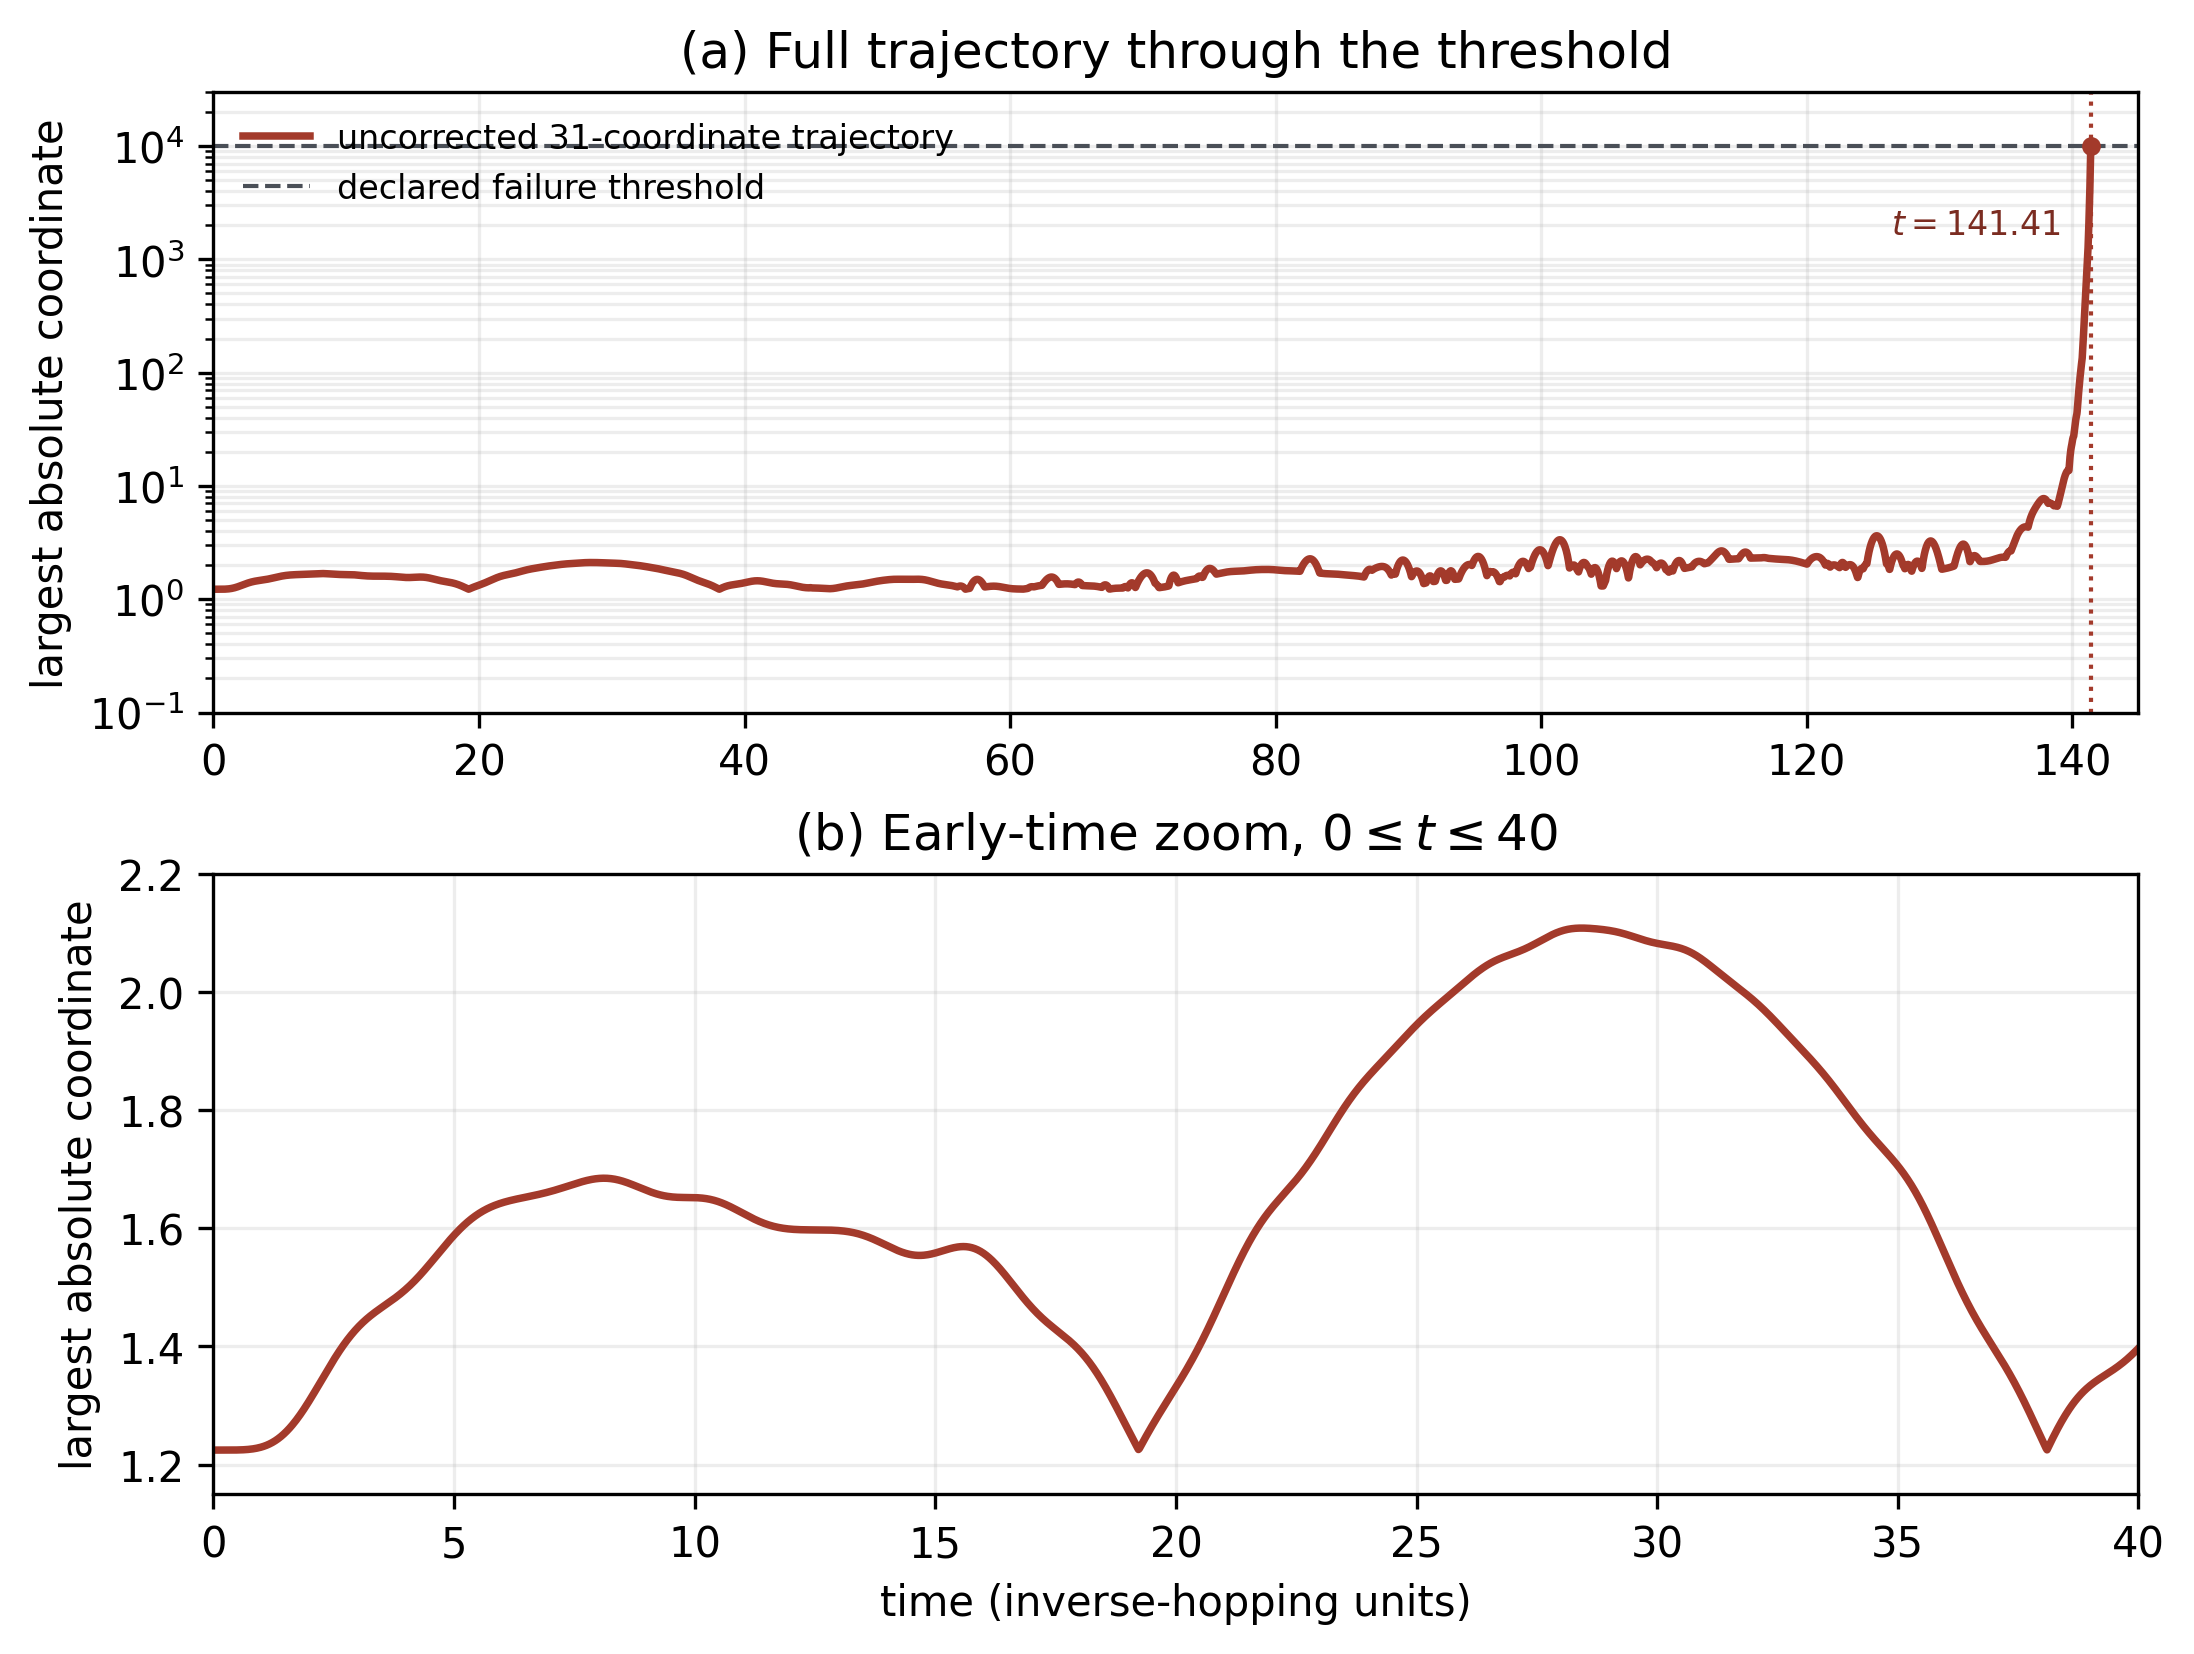
\includegraphics[width=\columnwidth]{advisor_project_overview_assets/paper_v/paper_v_divergence_reproduction_multiscale.pdf}
\caption{Uncorrected 31-coordinate archive trajectory.  Panel (a) shows the
full logarithmic-scale trajectory through the event
$\norm{x}_\infty=10^4$; panel (b) replots the same data over
$0\leq t\leq40\,t_{\rm hop}^{-1}$ with a linear vertical scale to resolve
the early oscillations.  At the threshold, the two largest correlation
coordinates reach $10^4$ and $8.99\times10^3$.}
\label{fig:divergence}
\end{figure}

\section{Joint Gram matrix and the admissible cone}

Let $r_a=\Tr(\rho\sigma_a)$ and
$\delta\sigma_a=\sigma_a-r_a\I_2$ for $a\in\{x,y,z\}$.  Form the centered
operator row
\begin{equation}
Y=(\delta b_0,\delta b_1,\delta b_0^\dagger,\delta b_1^\dagger,
\delta\sigma_x,\delta\sigma_y,\delta\sigma_z)
\label{eq:operator-row}
\end{equation}
and its Gram matrix $\mathcal G_{ab}=\langle Y_a^\dagger Y_b\rangle$.
The definitions in Eq.~\eqref{eq:moments}, bosonic commutation relations, and
the structural equalities give
\begin{equation}
\begin{aligned}
\langle\delta b_q^\dagger\delta b_r\rangle&=N_{rq},&
\langle\delta b_q\delta b_r\rangle&=A_{qr},\\
\langle\delta b_q\delta b_r^\dagger\rangle&=\delta_{qr}+N_{qr},&
\langle\delta b_q\delta\sigma_a\rangle&=c_{qa},\\
c_{qa}&=\Tr(C^q\sigma_a),&
E_{ab}&=\Tr(\rho\sigma_a\sigma_b)-r_ar_b.
\end{aligned}
\label{eq:gram-entries}
\end{equation}
Hence, for $c=(c_{qa})\in\C^{2\times3}$,
\begin{equation}
\begin{gathered}
\MB(N,A)=\begin{pmatrix}N^{\mathsf T}&A^*\\A&\I_2+N\end{pmatrix},
\qquad Z(C)=\begin{pmatrix}c^*\\c\end{pmatrix},\\
\boxed{\mathcal G(\rho,N,A,C)=
\begin{pmatrix}\MB&Z\\Z^\dagger&E\end{pmatrix}.}
\end{gathered}
\label{eq:joint-gram}
\end{equation}
The equality restrictions determine this block structure; positivity follows
from the Gram construction~\cite{hornJohnson2012}.  For every $z\in\C^7$,
\begin{equation}
z^\dagger\mathcal Gz
=\left\langle\left(\sum_a z_aY_a\right)^\dagger
\left(\sum_bz_bY_b\right)\right\rangle\geq0,
\label{eq:gram-psd-proof}
\end{equation}
so every physical state satisfies $\mathcal G\succeq0$.  If $\MB\succ0$,
block elimination gives the equivalent Schur condition
\begin{equation}
\mathcal G\succeq0
\Longleftrightarrow
\MB\succ0,\qquad E-Z^\dagger\MB^{-1}Z\succeq0.
\label{eq:schur}
\end{equation}
The second inequality is the joint operator Cauchy--Schwarz constraint that
bounds $C$ relative to its bosonic and electronic marginal moments.
Appendix~\ref{app:gram-schur} derives
Eqs.~\eqref{eq:gram-psd-proof}--\eqref{eq:schur} by expanding the Gram
quadratic form and completing the square~\cite{zhang2005}.

Let $\mathbb H_+^d=\{M\in\C^{d\times d}:M=M^\dagger,\ M\succeq0\}$ be the
fixed positive-semidefinite cone.  The tested representability domain is the
inverse image
\begin{equation}
\mathcal P=\{x:\rho(x),\I_2-\rho(x)\in\mathbb H_+^2,
\ \mathcal G(x)\in\mathbb H_+^7,
\ \Tr C^q(x)=0\}.
\label{eq:physical-domain}
\end{equation}
The matrix cone is fixed; the reconstructed matrices move through it as
$x(t)$ evolves.  Since $\MB$ is a principal submatrix of $\mathcal G$,
$\mathcal G\succeq0$ implies $\MB\succeq0$.\footnote{For
$u\in\C^4$, embed $u$ as $z=(u,0_3)\in\C^7$; then
$u^\dagger\MB u=z^\dagger\mathcal Gz\geq0$.  This is the
principal-submatrix inheritance property of Hermitian positive-semidefinite
matrices~\cite{hornJohnson2012}.}
In the trace-one dimer,
$\rho\succeq0$ also implies $\I_2-\rho\succeq0$ in exact arithmetic; both
electronic barriers were retained as independently evaluated numerical
constraints.  Fixed particle number supplies, with
$\widehat N_\uparrow=\sum_i c_{i\uparrow}^\dagger c_{i\uparrow}$,
\begin{equation}
\Tr C^q=\left\langle\delta b_q
\left(\widehat N_\uparrow-\Tr\rho\right)\right\rangle=0.
\label{eq:c-trace}
\end{equation}

Along the raw 31-coordinate trajectory,
\begin{equation}
\lambda_{\min}(\mathcal G)=0
\quad\text{first at}\quad
t=0.1607116782\,t_{\rm hop}^{-1}.
\label{eq:first-joint-crossing}
\end{equation}
At this event $\lambda(\rho)=(0.10380,0.89620)$ and
$\lambda_{\min}(\MB)=1.8890\times10^{-3}$; therefore the first failure
belongs to the joint electron--phonon cone while both marginal spectra remain
positive.  For $n$ phonon modes and any selected electronic operator family,
Eq.~\eqref{eq:gram-psd-proof} produces the corresponding larger Gram
constraint.  The reported numerical evidence specializes this construction
to the two-mode dimer.

\section{Differential cone constraints and the correction lift}

Let $M(t)=M(t)^\dagger$ have a simple minimum eigenpair
$M(t)v(t)=m(t)v(t)$ with $v^\dagger v=1$.  Differentiation and left
multiplication by $v^\dagger$ give the first-order boundary velocity
\begin{equation}
\dot m(t)=v(t)^\dagger\dot M(t)v(t).
\label{eq:eigenvalue-velocity}
\end{equation}
This is the standard simple-eigenvalue perturbation formula~\cite{kato1966}.
A negative value at $m=0$ points out of $\mathbb H_+^d$.  We impose
the exponential semidefinite matrix barrier\footnote{Equation~\eqref{eq:matrix-barrier}
is the complex-Hermitian analogue of the exponential semidefinite matrix
barrier condition of Ong et al.~\cite[Proposition~1]{ong2025}.  Their
$\dot H\succeq-c_\alpha H$ becomes Eq.~\eqref{eq:matrix-barrier} under
$H=M-h_\star I_d$ and $c_\alpha=\beta$; Eq.~\eqref{eq:barrier-bound} then
follows by the displayed integrating-factor argument.}
\begin{equation}
\dot M+\beta(M-h_\star\I_d)\succeq0,
\qquad \beta=5,\quad h_\star=10^{-5}.
\label{eq:matrix-barrier}
\end{equation}
Its scalar restriction obeys
\begin{equation}
\dot m+\beta(m-h_\star)\geq0
\Longrightarrow
m(t)\geq h_\star+[m(0)-h_\star]e^{-\beta t},
\label{eq:barrier-bound}
\end{equation}
obtained by multiplying by $e^{\beta t}$ and integrating.  At
$m=h_\star$ it requires $\dot m\geq0$; in the interior it permits controlled
motion toward the boundary.

At one right-hand-side evaluation, let $\dot x_0=f(t,x)$ and add
$w=(w_0,\ldots,w_{30})\in\R^{31}$ to this velocity.  Lowercase $\delta$
denotes a centered operator, as in $\delta b_q=b_q-B_q$.  Throughout the
correction construction,
$\Delta\dot Y(w):=\dot Y_{\rm c}-\dot Y_0$ denotes the velocity increment
induced in a reconstructed block $Y$ by $w$.  Its block lift is the derivative
of Eqs.~\eqref{eq:rho-reconstruction}--\eqref{eq:c-reconstruction}:
\begin{equation}
\Delta\dot\rho=
\begin{pmatrix}w_0/2&w_1+\ii w_2\\w_1-\ii w_2&-w_0/2\end{pmatrix},
\quad
\Delta\dot B=\binom{w_3+\ii w_4}{w_5+\ii w_6},
\label{eq:lift-rho-b}
\end{equation}
\begin{equation}
\begin{gathered}
\Delta\dot N=
\begin{pmatrix}w_7&w_9+\ii w_{10}\\w_9-\ii w_{10}&w_8\end{pmatrix},\\[2pt]
\Delta\dot A=
\begin{pmatrix}
w_{11}+\ii w_{12}&w_{15}+\ii w_{16}\\
w_{15}+\ii w_{16}&w_{13}+\ii w_{14}
\end{pmatrix}
\end{gathered}
\label{eq:lift-na}
\end{equation}
The correlation lift is
{\scriptsize
\begin{equation}
\begin{aligned}
\Delta\dot C^0&=
\begin{pmatrix}
\frac{w_{17}+\ii w_{18}+w_{19}+\ii w_{20}}2&w_{21}+\ii w_{22}\\
w_{23}+\ii w_{24}&\frac{w_{17}+\ii w_{18}-w_{19}-\ii w_{20}}2
\end{pmatrix},\\
\Delta\dot C^1&=
\begin{pmatrix}
\frac{w_{17}+\ii w_{18}+w_{25}+\ii w_{26}}2&w_{27}+\ii w_{28}\\
w_{29}+\ii w_{30}&\frac{w_{17}+\ii w_{18}-w_{25}-\ii w_{26}}2
\end{pmatrix}.
\end{aligned}
\label{eq:lift-c}
\end{equation}}
Consequently
\begin{equation}
\Delta\dot\MB=
\begin{pmatrix}\Delta\dot N^{\mathsf T}&\Delta\dot A^*\\
\Delta\dot A&\Delta\dot N\end{pmatrix}.
\label{eq:lift-mb}
\end{equation}
With $\Delta r_a=\Tr(\Delta\dot\rho\,\sigma_a)$ and
$\Delta c_{qa}=\Tr(\Delta\dot C^q\sigma_a)$,
\begin{equation}
\begin{aligned}
(\Delta\dot E)_{ab}
&=\Tr(\Delta\dot\rho\,\sigma_a\sigma_b)
-\Delta r_ar_b-r_a\Delta r_b,\\
\Delta\dot Z&=\binom{\Delta c^*}{\Delta c},\\
\Delta\dot{\mathcal G}(w)&=
\begin{pmatrix}\Delta\dot\MB&\Delta\dot Z\\
\Delta\dot Z^\dagger&\Delta\dot E\end{pmatrix}.
\end{aligned}
\label{eq:joint-lift}
\end{equation}
This lift changes representation but introduces no additional degrees of
freedom.

Let $s=\Tr C^0=\Tr C^1$ and let $E_{\rm int}$ be the time-independent
internal-energy functional
\begin{equation}
\begin{aligned}
E_{\rm int}(X)={}&\nu\Tr(h_0\rho)
+\omega_{\rm ph}(B^\dagger B+\Tr N)\\
&+2\nu\Re\sum_{qij}(G_q)_{ij}
(B_q\rho_{ji}+C^q_{ji}),\\
h_0={}&\begin{pmatrix}0&-t_{\rm hop}\\-t_{\rm hop}&0\end{pmatrix}.
\end{aligned}
\label{eq:internal-energy}
\end{equation}
Equation~\eqref{eq:internal-energy} contains the time-independent internal
energy; drive work enters separately through $V(t)$.  The correction is the
convex semidefinite program~\cite{vandenbergheBoyd1996}
{\footnotesize
\begin{equation}
\begin{aligned}
w^*=\arg\min_{w\in\R^{31}}\quad&\tfrac12\norm{w}_2^2\\
\text{subject to}\quad
&\dot\rho_0+\Delta\dot\rho(w)+\beta(\rho-h_\star\I_2)\succeq0,\\
&-\dot\rho_0-\Delta\dot\rho(w)
+\beta(\I_2-\rho-h_\star\I_2)\succeq0,\\
&\dot{\mathcal G}_0+\Delta\dot{\mathcal G}(w)
+\beta(\mathcal G-h_\star\I_7)\succeq0,\\
&\dot s_0+w_{17}+\ii w_{18}+\beta s=0,\\
&\nabla_xE_{\rm int}(x)^{\mathsf T}w=0.
\end{aligned}
\label{eq:correction-sdp}
\end{equation}}%
\footnote{The first two matrix inequalities retain the spectrum of $\rho$ in
$[h_\star,1-h_\star]$; the third retains the joint Gram matrix in its
positive-semidefinite cone; the fourth enforces the fixed-number correlation
trace; and the fifth makes the correction tangent to an internal-energy level
set.  Appendix~\ref{app:constraint-origin} gives their derivation.}
The complex trace condition is two real equalities and gives
$\dot s=-\beta s$.  The last equality sets the correction-induced energy
flux to zero while retaining the physical work performed by $V(t)$.  The
Euclidean objective selects the smallest coordinate-space velocity change in
the displayed scaling; its lifted-matrix metric differs from the Frobenius
metric.  The corrected vector
field is
\begin{equation}
f_{\rm c}(t,x)=f(t,x)+w^*(t,x).
\label{eq:corrected-field}
\end{equation}

\subsection{Null-space cutting-plane solution and RK4}

Let $e_j\in\R^{31}$ select the zero-based coordinate $w_j$.  The energy row
and the real and imaginary trace rows of Eq.~\eqref{eq:correction-sdp} are
\begin{equation}
\begin{aligned}
L_{\rm eq}w&=d_{\rm eq},\\
L_{\rm eq}&=\begin{pmatrix}
\nabla_xE_{\rm int}^{\mathsf T}\\ e_{17}^{\mathsf T}\\e_{18}^{\mathsf T}
\end{pmatrix},\\
d_{\rm eq}&=\begin{pmatrix}
0\\-\Re(\dot s_0+\beta s)\\-\Im(\dot s_0+\beta s)
\end{pmatrix}.
\end{aligned}
\label{eq:equality-system}
\end{equation}
An SVD equality elimination~\cite{boydVandenberghe2004} yields
\begin{equation}
\begin{gathered}
w_{\rm p}=L_{\rm eq}^+d_{\rm eq},\qquad L_{\rm eq}Z=0,
\qquad Z^\mathsf TZ=\I,\\
w=w_{\rm p}+Zy
\end{gathered}
\label{eq:nullspace}
\end{equation}
where $w_{\rm p}\perp\operatorname{range}Z$.  The columns of $Z$
orthonormalize the equality-feasible tangent directions in the chosen
Euclidean coordinate metric.  Whitening would additionally transform a
nontrivial covariance or metric.  Therefore
\begin{equation}
\norm{w}_2^2=\norm{w_{\rm p}}_2^2+\norm y_2^2,
\label{eq:nullspace-norm}
\end{equation}
and the remaining minimum-norm problem is in $y$.  For the barrier sectors
$\ell\in\{\rho^-,\rho^+,\mathcal G\}$, the affine pieces inherited directly
from Eq.~\eqref{eq:correction-sdp} are
{\scriptsize
\begin{equation}
\begin{array}{c|c|c}
\ell&M_{0,\ell}&\Delta M_\ell(w)\\ \hline
\rho^-&\dot\rho_0+\beta(\rho-h_\star\I_2)&\Delta\dot\rho(w)\\
\rho^+&-\dot\rho_0+\beta(\I_2-\rho-h_\star\I_2)&-\Delta\dot\rho(w)\\
\mathcal G&\dot{\mathcal G}_0+\beta(\mathcal G-h_\star\I_7)
&\Delta\dot{\mathcal G}(w)
\end{array}
\label{eq:barrier-pieces}
\end{equation}}
Define
\begin{equation}
B_\ell(y)=M_{0,\ell}+\Delta M_\ell(w_{\rm p}+Zy).
\label{eq:affine-barrier}
\end{equation}
If $B_\ell(y^{(k)})v=\lambda v$ with $\lambda<0$ and $v^\dagger v=1$, let
\begin{equation}
[a_\ell(v)]_j=v^\dagger\Delta M_\ell(e_j)v,\qquad
n=Z^\mathsf Ta_\ell(v).
\label{eq:cut-normal}
\end{equation}
Because $B_\ell$ is affine,
\begin{equation}
v^\dagger B_\ell(y)v
=\lambda+n^\mathsf T(y-y^{(k)})\geq0
\Longleftrightarrow
n^\mathsf Ty\geq n^\mathsf Ty^{(k)}-\lambda.
\label{eq:eigenvector-cut}
\end{equation}
Each negative eigenvector therefore supplies an exact half-space containing
the semidefinite feasible set.  After $p$ exposed modes, SLSQP solves
\begin{equation}
\min_y\tfrac12y^\mathsf Ty
\quad\text{subject to}\quad n_i^\mathsf Ty\geq c_i,
\quad i=1,\ldots,p.
\label{eq:cutting-plane-qp}
\end{equation}
The algorithm reconstructs $w$, diagonalizes all three complete barrier
matrices, appends any newly violated eigenvector cut, and repeats.  A direct
spectral SLSQP solve is the fallback near degenerate boundaries.

The controller is evaluated inside, rather than after, the Runge--Kutta
stages.  For $h=0.01\,t_{\rm hop}^{-1}$,
\begin{equation}
\begin{aligned}
k_1&=f_{\rm c}(t_n,x_n),\\
k_2&=f_{\rm c}(t_n+h/2,x_n+hk_1/2),\\
k_3&=f_{\rm c}(t_n+h/2,x_n+hk_2/2),\\
k_4&=f_{\rm c}(t_n+h,x_n+hk_3),\\
x_{n+1}&=x_n+\frac h6(k_1+2k_2+2k_3+k_4).
\end{aligned}
\label{eq:corrected-rk4}
\end{equation}
Each $k_i$ uses a fresh matrix reconstruction and a fresh solve of
Eq.~\eqref{eq:correction-sdp}.  Thus the $t=1000$ trajectory contains
$100{,}000$ RK4 steps and $400{,}000$ constrained velocity evaluations.

\section{Representability and accuracy}

Over $0\leq t\leq4\,t_{\rm hop}^{-1}$, the exact, raw, and corrected
minimum eigenvalues are
\begin{table}[H]
\centering
\scriptsize
\begin{tabular}{@{}lccc@{}}
\toprule
route & $\min\lambda(\mathcal G)$ & $\min\lambda(\MB)$
& $[\min\lambda(\rho),\max\lambda(\rho)]$\\
\midrule
exact & $2.8524\!\times\!10^{-5}$ & $2.8549\!\times\!10^{-5}$
& $[0.08338,0.91662]$\\
raw & $-0.51727$ & $-0.14777$ & $[-0.02230,1.02230]$\\
corrected & $2.0637\!\times\!10^{-5}$ & $2.0647\!\times\!10^{-5}$
& $[0.02395,0.97605]$\\
\bottomrule
\end{tabular}
\caption{Physicality certificates over the driven interval.}
\label{tab:physicality}
\end{table}

\begin{figure}[H]
\centering
\includegraphics[width=\columnwidth]{advisor_project_overview_assets/paper_v/paper_v_physicality_correction.pdf}
\caption{The raw closure leaves the joint Gram cone; exact cutoff-16 and
corrected trajectories retain nonnegative joint eigenvalues over the shown
interval.}
\label{fig:physicality}
\end{figure}

The corrected fixed-step trajectory through $t=1000\,t_{\rm hop}^{-1}$
satisfied
\begin{equation}
\begin{aligned}
\min_t\lambda_{\min}(\mathcal G)&=2.06367\times10^{-5},\\
\min_t\lambda_{\min}(\MB)&=2.06469\times10^{-5},\\
0.0239455\leq\lambda_{\min}(\rho)
&\leq\lambda_{\max}(\rho)\leq0.976055,\\
\max_{t,j}|x_j(t)|&=2.09860,\\
\max_{t,q}|\Tr C^q(t)|&=8.78\times10^{-17}.
\end{aligned}
\label{eq:long-horizon}
\end{equation}
All $400{,}000$ correction solves converged; the largest $\norm{w^*}_2$ was
$0.345567$.  The maximum correction-induced energy flux was
$2.64\times10^{-16}$, and
\begin{equation}
\max_{4\leq t\leq1000}|E_{\rm int}(t)-E_{\rm int}(4)|
=5.03\times10^{-6}.
\label{eq:energy-result}
\end{equation}
The Gaussian drive retains a negligible analytic tail after $t=4$;
Eq.~\eqref{eq:energy-result} therefore combines numerical drift with its
residual work.

Representability and trajectory accuracy are distinct diagnostics.  The
subscript ``ex'' denotes contractions of the exact cutoff-16 wavefunction,
while ``r'' and ``c'' denote the raw and corrected archive trajectories.  For
$Y\in\{\rho,B,N,A,C\}$, define
\begin{equation}
\begin{aligned}
D_Y(T)&=\left[\frac1T\int_0^T
\norm{Y_{\rm ex}(t)-Y_{\rm ex}(0)}_{\rm F}^2dt\right]^{1/2},\\
e_Y^{(a)}(t;T)&=\frac{\norm{Y_a(t)-Y_{\rm ex}(t)}_{\rm F}}{D_Y(T)},\\
\varepsilon_Y^{(a)}(T)&=
\left[\frac1T\int_0^T\bigl(e_Y^{(a)}(t;T)\bigr)^2dt\right]^{1/2},
\quad a\in\{\mathrm r,\mathrm c\}.
\end{aligned}
\label{eq:trajectory-error}
\end{equation}
Thus $e_Y^{(a)}$ is the instantaneous block error in units of the exact
block's own RMS motion, and $\varepsilon_Y^{(a)}$ is its time-RMS.  Over the
common early interval $T=4$, the measured errors were
\begin{table}[H]
\centering
\small
\begin{tabular}{@{}lcc@{}}
\toprule
block $Y$ & $\varepsilon_Y^{(\mathrm r)}$
& $\varepsilon_Y^{(\mathrm c)}$\\
\midrule
$\rho$ & 0.6072 & 0.7613\\
$B$    & 0.1076 & 0.2089\\
$N$    & 6.5530 & 8.5389\\
$A$    & 4.8673 & 4.6735\\
$C$    & 2.5749 & 2.1250\\
\bottomrule
\end{tabular}
\caption{Dynamic-normalized RMS trajectory errors over $0\leq t\leq4$.}
\label{tab:accuracy}
\end{table}
The correction changes the $A$ and $C$ errors from $4.8673$ to $4.6735$ and
from $2.5749$ to $2.1250$, respectively.  The $\rho$, $B$, and $N$ errors
increase from $0.6072$ to $0.7613$, from $0.1076$ to $0.2089$, and from
$6.5530$ to $8.5389$.  This mixed outcome reflects the objective of the
controller: it enforces representability rather than minimizing trajectory
error against the exact reference.

For the long-horizon reference, DOP853 propagated the driven cutoff-16
wavefunction through $t=10$; sparse exponentiation of the static Hamiltonian
then propagated it through $t=1000$.  The omitted drive amplitude after
$t=10$ is bounded by $3.86\times10^{-22}$.  Against an uninterrupted DOP853
calculation through $t=20$, this split route agreed in all 31 coordinates to
$2.45\times10^{-12}$.  This is a matched cutoff-16 reference, not a claim of
phonon-cutoff convergence at $t=1000$.

The archive reports site occupation and the electronic, phonon,
electron--phonon, and total-energy contributions, so
Fig.~\ref{fig:archive-observable-trajectories} uses the same observable
family.  In the trace-one dimer, its polarization
$P=(\rho_{22}-\rho_{11})/2=1/2-\rho_{11}$ contains no information beyond the
plotted $\rho_{11}$.  The raw RK4 trajectory was step-refined to $h=0.005$
and terminates at $t=141.4001$; this agrees with the adaptive event time
$141.4059$ in Eq.~\eqref{eq:divergence-time}.  The corrected $h=0.01$
trajectory and exact reference continue through $t=1000$.

\begin{figure*}[t]
\centering
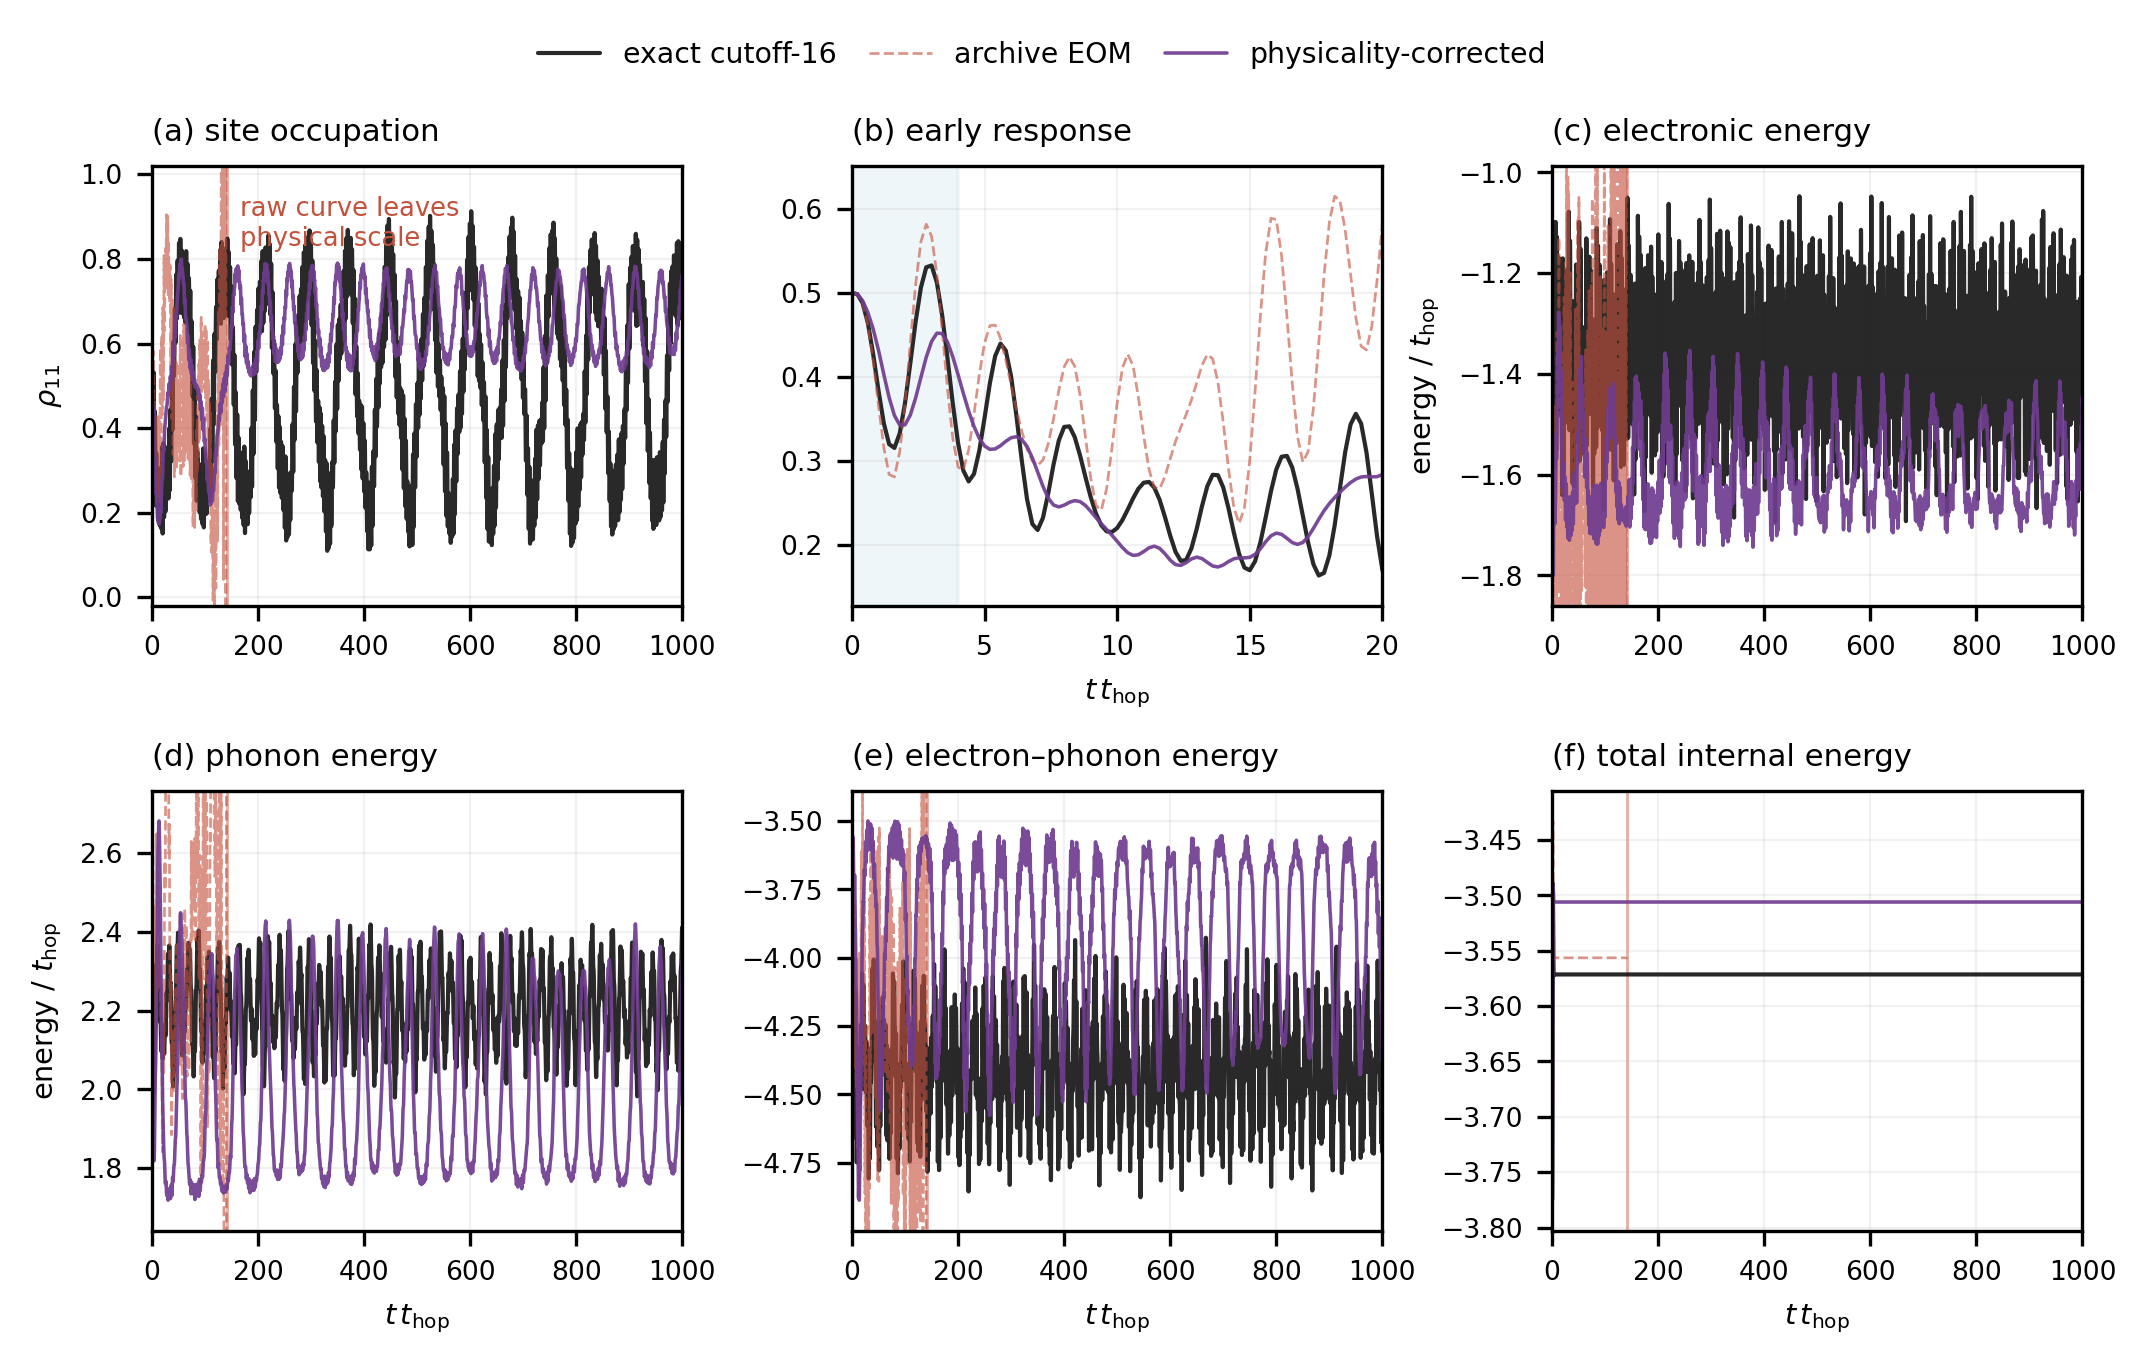
\includegraphics[width=0.98\textwidth]{advisor_project_overview_assets/paper_v/paper_v_archive_observable_trajectories.pdf}
\caption{Archive-style physical observables over the complete tested horizon.
Black is exact cutoff-16 Hamiltonian propagation, dashed red is the raw
archive closure, and purple is the online physicality-corrected closure.
Panel (b) expands the first 20 time units; its blue band marks $0\leq t\leq4$.
The vertical red line marks the raw amplitude-threshold event.  The component
panels retain scales set by the exact and corrected trajectories, so the raw
component energies visibly leave the plotted physical range before their
terminal blow-up.  Their cancellation in panel (f) shows why conserved total
energy alone cannot certify accurate component dynamics.}
\label{fig:archive-observable-trajectories}
\end{figure*}

\subsection{Post-pulse spectral accuracy}

To distinguish oscillation-frequency content from accumulated phase error, I
Fourier analyzed the same observables on the fixed common interval
$10\leq t\leq120\,t_{\rm hop}^{-1}$, which starts after the drive and ends
before the raw terminal growth.  For each mean-subtracted observable $O_a$,
$a\in\{\mathrm{ex},\mathrm r,\mathrm c\}$, a Hann window $h_n$ gives the
normalized positive-frequency power and its distance from the exact spectrum,
\begin{equation}
\begin{aligned}
p_a^O(\omega_k)&=
\frac{\left|\sum_n h_n[O_a(t_n)-\bar O_a]
e^{-\ii\omega_kt_n}\right|^2}
{\sum_{\ell>0}\left|\sum_n h_n[O_a(t_n)-\bar O_a]
e^{-\ii\omega_\ell t_n}\right|^2},\\
H_a^O&=\left[\frac12\sum_{k>0}
\left(\sqrt{p_a^O(\omega_k)}-
\sqrt{p_{\rm ex}^O(\omega_k)}\right)^2\right]^{1/2}.
\end{aligned}
\label{eq:spectral-distance}
\end{equation}
Here $H=0$ denotes identical normalized power spectra.  The correction changes
$H$ from $0.6870$ to $0.2154$ for the site occupation, but from $0.8256$ to
$0.8854$, $0.7022$ to $0.8198$, and $0.7406$ to $0.8524$ for the electronic,
phonon, and electron--phonon energies, respectively.  These four orderings are
unchanged when the common-window endpoint is varied among $80$, $100$, and
$120\,t_{\rm hop}^{-1}$.

The oscillation-amplitude ratios
$\operatorname{RMS}(O_a-\bar O_a)/\operatorname{RMS}(O_{\rm ex}-\bar O_{\rm ex})$
change from $0.8714$ to $0.8484$ for occupation, from $2.7373$ to $0.9053$
for electronic energy, from $3.1432$ to $2.6147$ for phonon energy, and from
$2.7455$ to $2.0862$ for electron--phonon energy.  Thus the correction greatly
improves the component-energy amplitude scale but not their distribution of
spectral weight.  On the higher-resolution exact--corrected interval
$10\leq t\leq1000\,t_{\rm hop}^{-1}$, the corresponding corrected spectral
distances are $0.9663$, $0.9773$, $0.9875$, and $0.9886$; bounded propagation
therefore does not imply long-time spectral agreement.  Total internal energy
is omitted because its post-pulse signal is constant to the reported numerical
precision and consequently carries only a zero-frequency component.

\begin{figure*}[t]
\centering
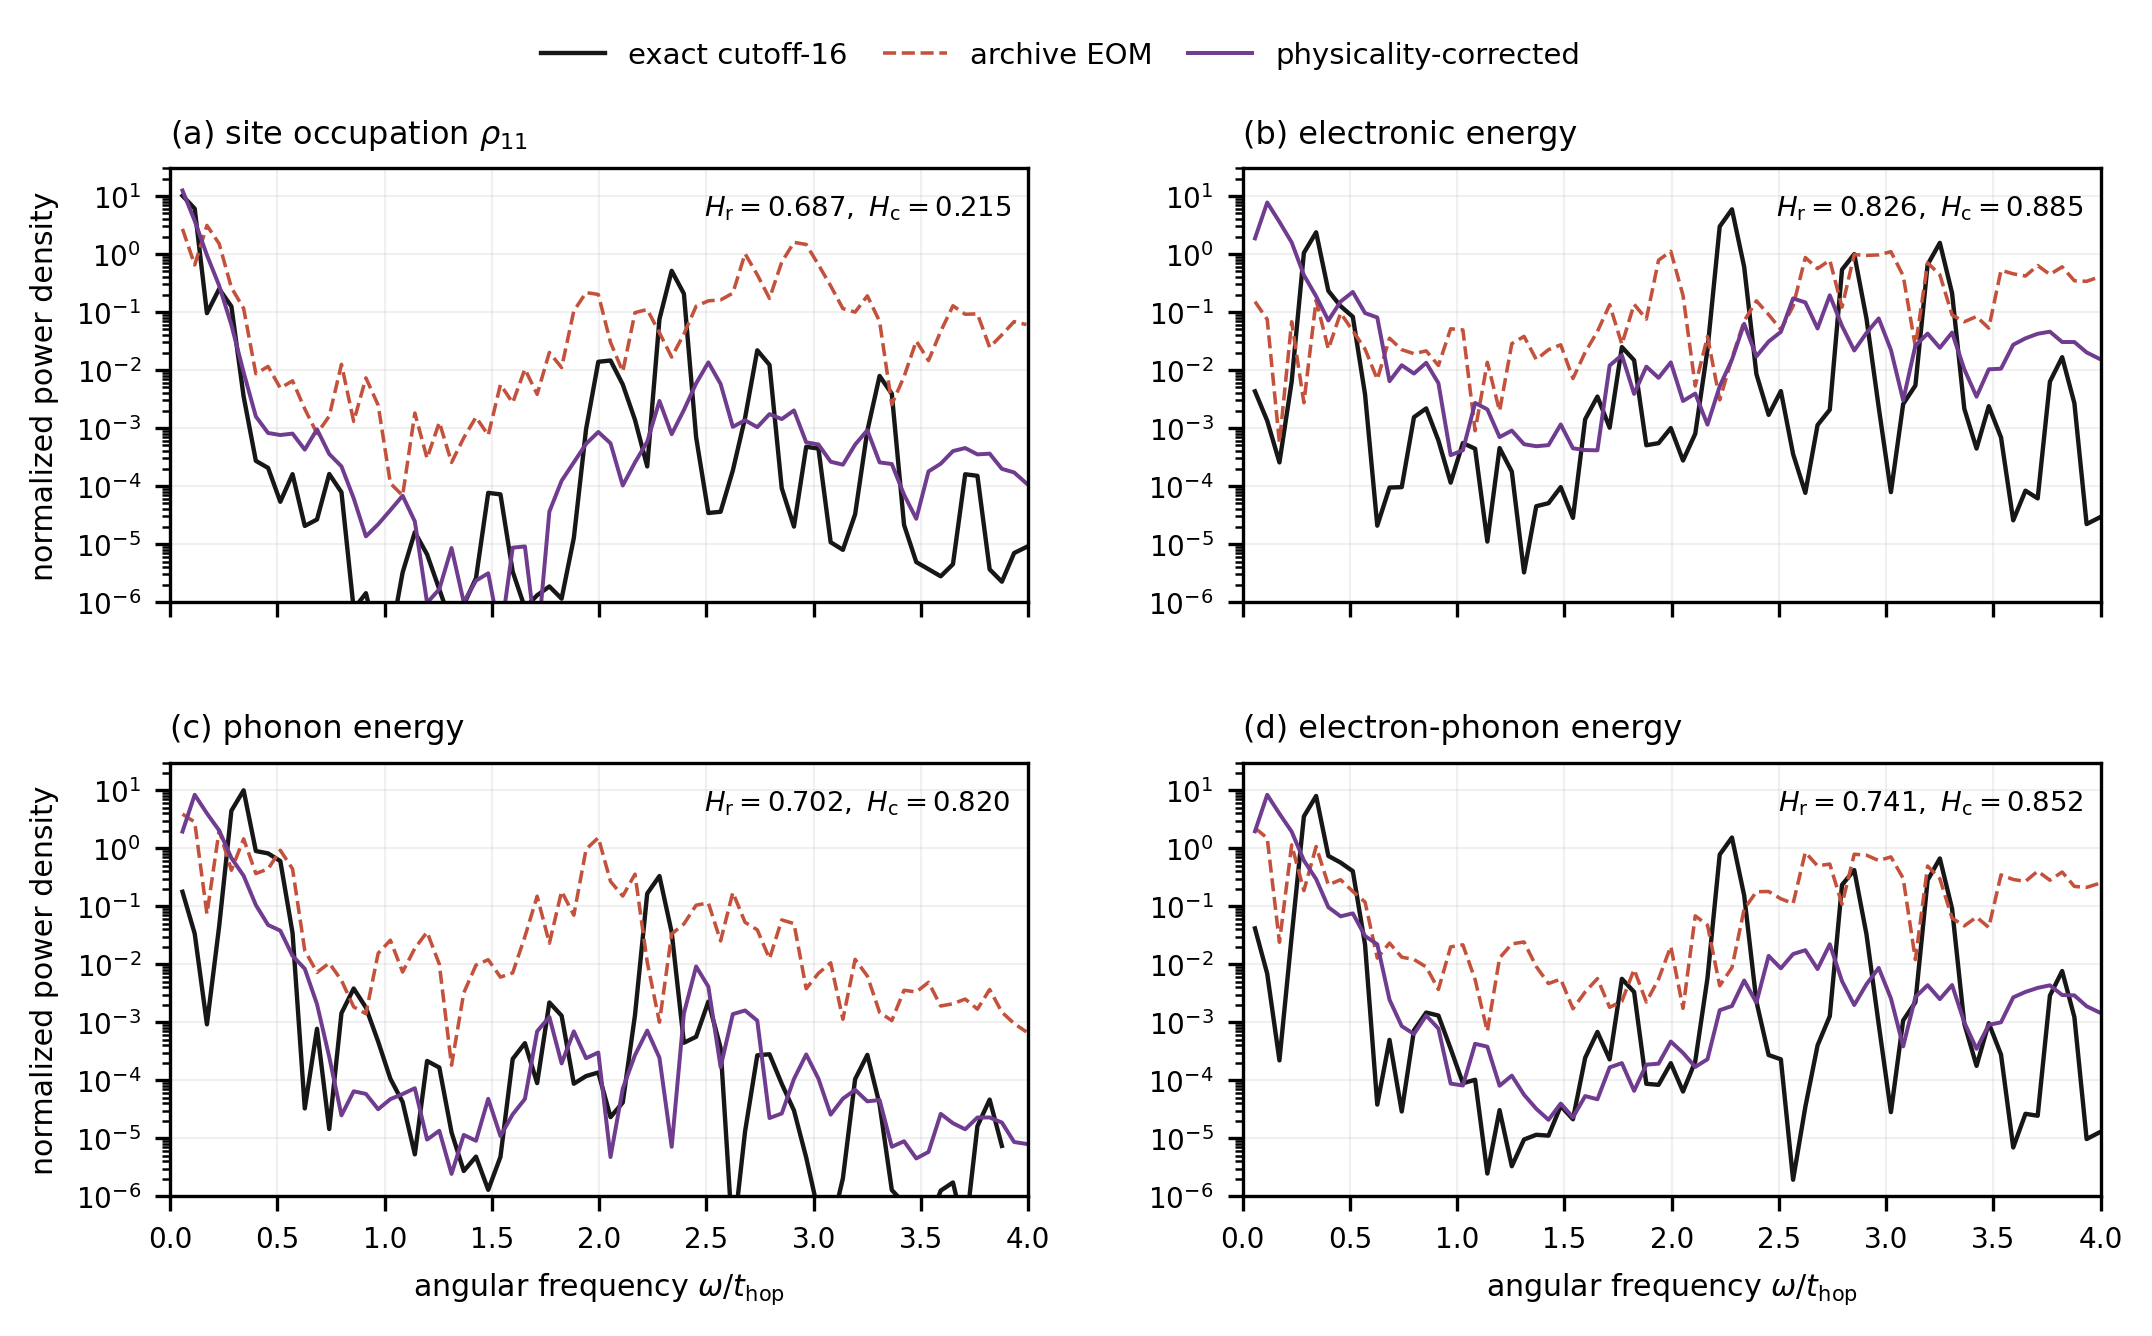
\includegraphics[width=0.98\textwidth]{advisor_project_overview_assets/paper_v/paper_v_archive_observable_spectra.pdf}
\caption{Normalized post-pulse power spectra on the matched interval
$10\leq t\leq120\,t_{\rm hop}^{-1}$, sampled every
$0.2\,t_{\rm hop}^{-1}$.  Black is exact cutoff-16 propagation, dashed red is
the raw archive closure, and purple is the physicality-corrected closure.
The displayed band $0<\omega\leq4\,t_{\rm hop}$ contains more than $99.8\%$
of the exact power in every panel; the annotated Hellinger distances use the
complete positive-frequency spectrum from Eq.~\eqref{eq:spectral-distance}.
The correction improves the occupation spectrum, while the component-energy
spectral shapes remain inaccurate.}
\label{fig:archive-observable-spectra}
\end{figure*}

To test whether the coordinate metric, rather than the constraints, limited
the corrected accuracy, I repeated the matched calculation through $t=20$
with the same feasible set but replaced the Euclidean objective by the
lifted-Frobenius objective
\begin{equation}
\begin{aligned}
J_{\rm F}(w)=\tfrac12\bigl(&\norm{\Delta\dot\rho(w)}_{\rm F}^2
+\norm{\Delta\dot B(w)}_2^2+\norm{\Delta\dot N(w)}_{\rm F}^2\\
&+\norm{\Delta\dot A(w)}_{\rm F}^2
+\textstyle\sum_q\norm{\Delta\dot C^q(w)}_{\rm F}^2\bigr).
\end{aligned}
\label{eq:frobenius-objective}
\end{equation}
This minimizes the total squared size of the five lifted matrix-block
corrections, whereas Eq.~\eqref{eq:correction-sdp} minimizes the 31 real
coordinate entries in their chosen scaling.

The matched metric ablation supplies a four-way finite-horizon spectral
comparison on $0\leq t\leq20\,t_{\rm hop}^{-1}$.  For site occupation,
electronic energy, phonon energy, and electron--phonon energy, respectively,
the Hellinger distances $(H_{\rm r},H_{\rm E},H_{\rm F})$ for the raw,
Euclidean-corrected, and lifted-Frobenius-corrected trajectories are
$(0.2557,0.4063,0.3849)$, $(0.4539,0.6378,0.6215)$,
$(0.4431,0.0934,0.0898)$, and $(0.2528,0.3407,0.3330)$.  The
lifted-Frobenius metric therefore gives a small spectral-shape improvement
over the Euclidean metric in all four observables, while both corrections
improve on the raw closure only for the phonon-energy spectrum.  These
orderings are unchanged on the restricted interval
$4\leq t\leq20\,t_{\rm hop}^{-1}$.

\begin{figure*}[t]
\centering
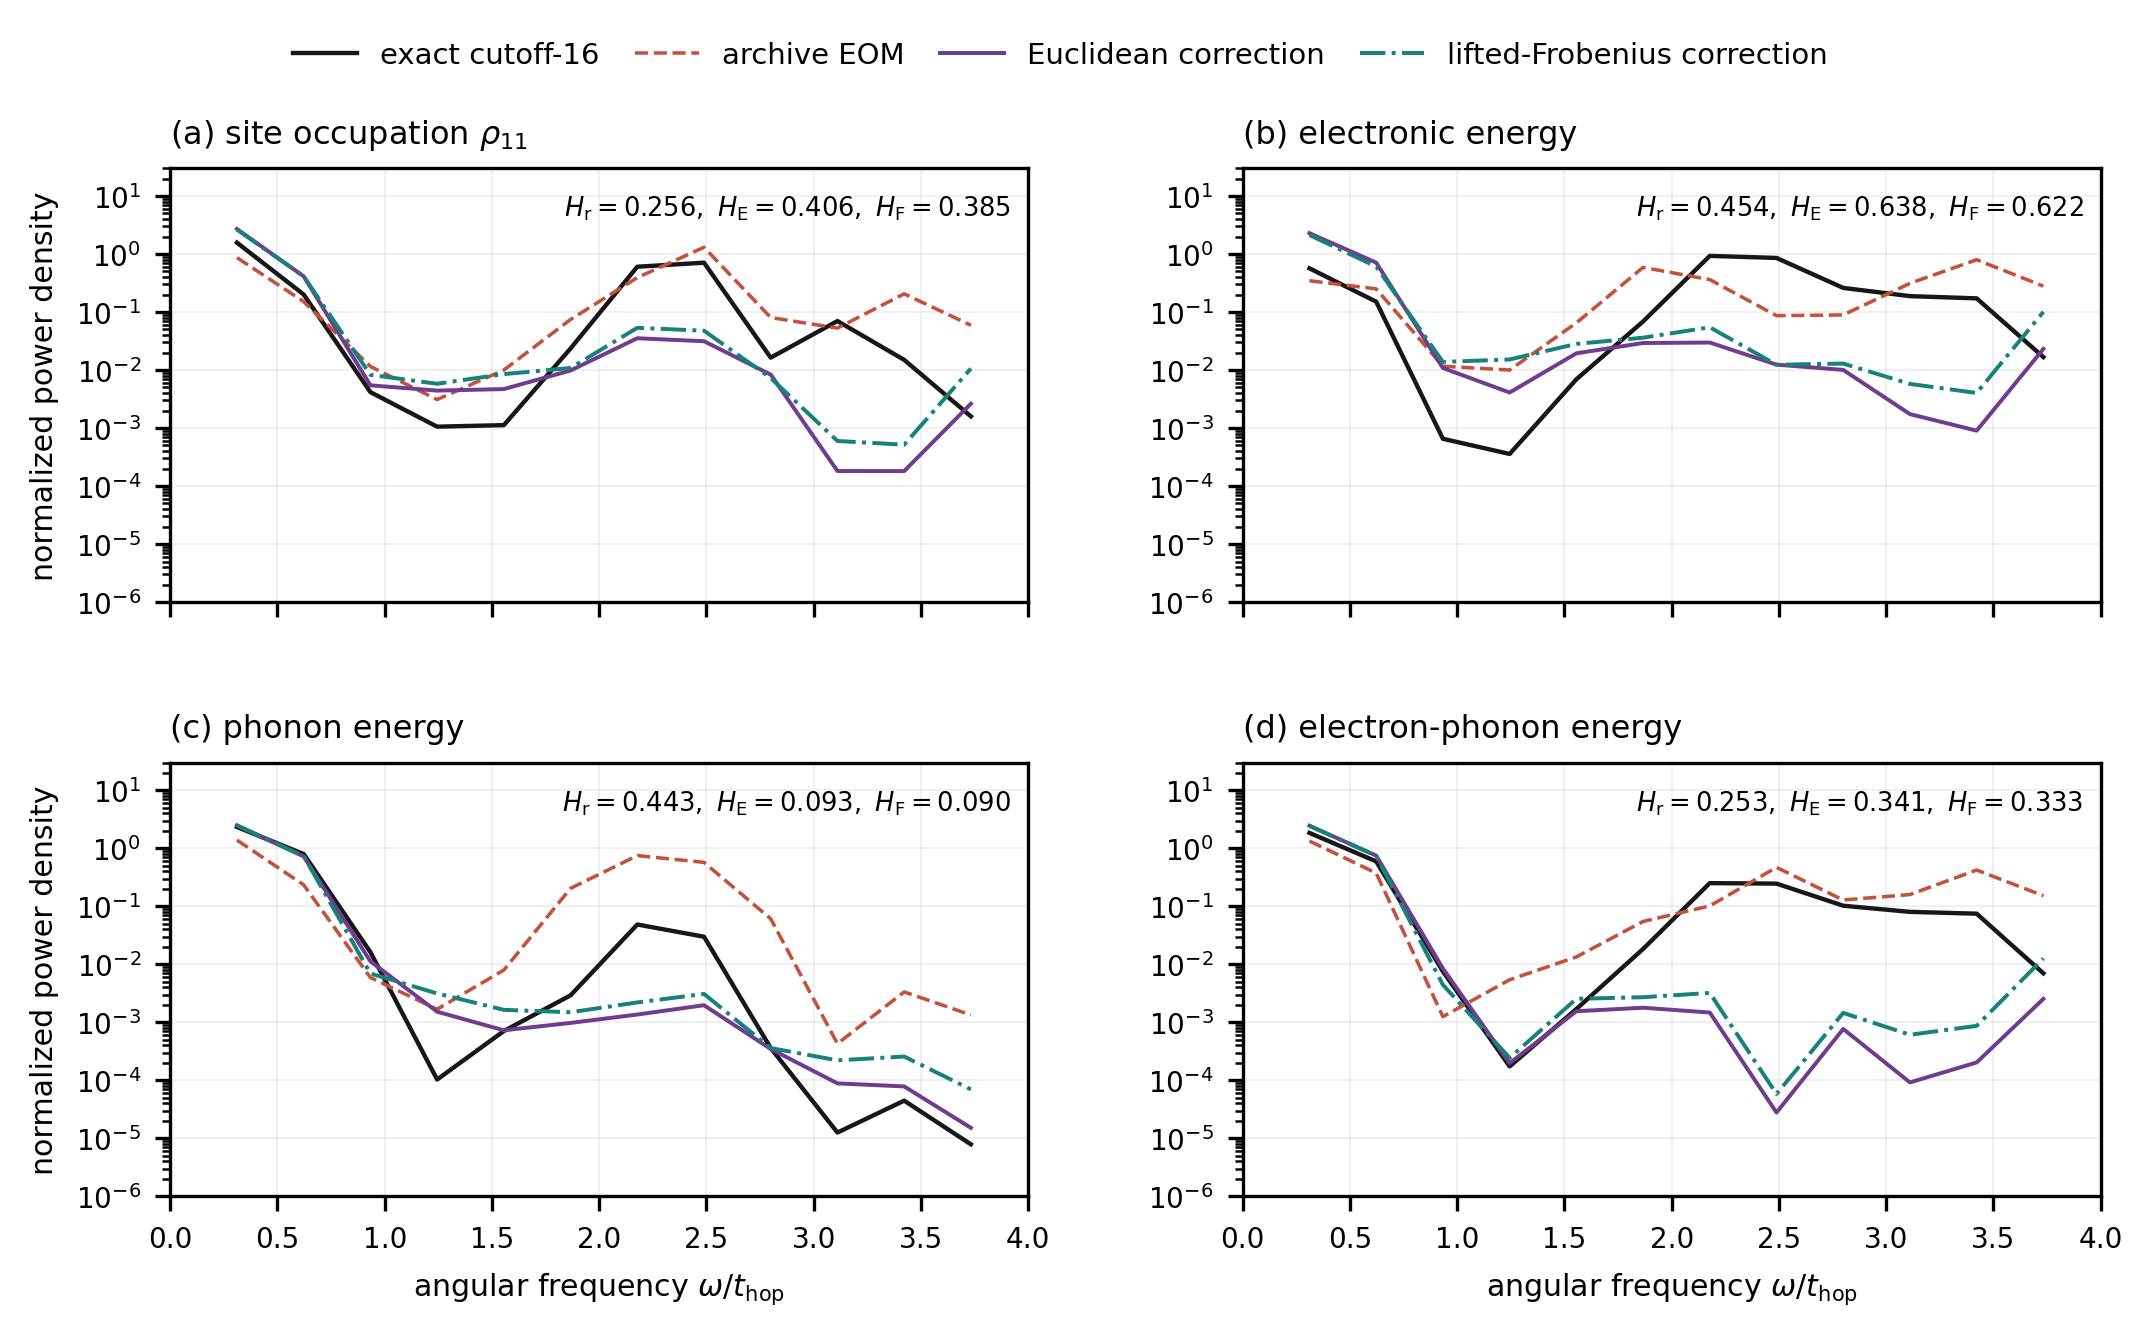
\includegraphics[width=0.98\textwidth]{advisor_project_overview_assets/paper_v/paper_v_archive_observable_spectra_metric_t20.pdf}
\caption{Finite-horizon correction-metric spectra on the matched interval
$0\leq t\leq20\,t_{\rm hop}^{-1}$, sampled every
$0.2\,t_{\rm hop}^{-1}$.  Black is exact cutoff-16 propagation, dashed red is
the raw archive closure, purple is the Euclidean correction, and dash-dotted
teal is the lifted-Frobenius correction.  Each panel reports the complete
positive-frequency Hellinger distances $H_{\rm r}$, $H_{\rm E}$, and
$H_{\rm F}$ from the exact normalized spectrum.}
\label{fig:archive-observable-spectra-metric}
\end{figure*}

\begin{figure*}[t]
\centering
\includegraphics[width=0.98\textwidth]{advisor_project_overview_assets/paper_v/paper_v_correction_metric_observables_t20.pdf}
\caption{Correction-metric comparison over
$0\leq t\leq20\,t_{\rm hop}^{-1}$.  Black is exact cutoff-16 propagation,
dashed red is the raw archive closure, purple is the Euclidean correction,
and dash-dotted teal is the lifted-Frobenius correction.  Panel (f) shows
absolute internal-energy error against the exact reference; the blue bands
mark $0\leq t\leq4$.}
\label{fig:archive-observable-trajectories-short}
\end{figure*}

Figure~\ref{fig:block-error-trajectories} retains the full time dependence of
the matrix errors.  Its time axis is linear through $t=4$ and logarithmic
thereafter, so both the early accuracy cost in Table~\ref{tab:accuracy} and
the terminal raw divergence remain visible.  For $T=1000$, the corrected
time-RMS values $\varepsilon_Y^{(\mathrm c)}$ in the order
$(\rho,B,N,A,C)$ are
$(1.1951,1.2173,1.2761,1.2088,1.1733)$.  The correction therefore does not
repair the inaccurate closure: it keeps all five errors finite and of the
same order as the exact dynamics while the raw errors diverge.  In particular,
the statement that the correction raises the $\rho$, $B$, and $N$ errors is
an early-window statement, not a full-horizon average.

\begin{figure*}[t]
\centering
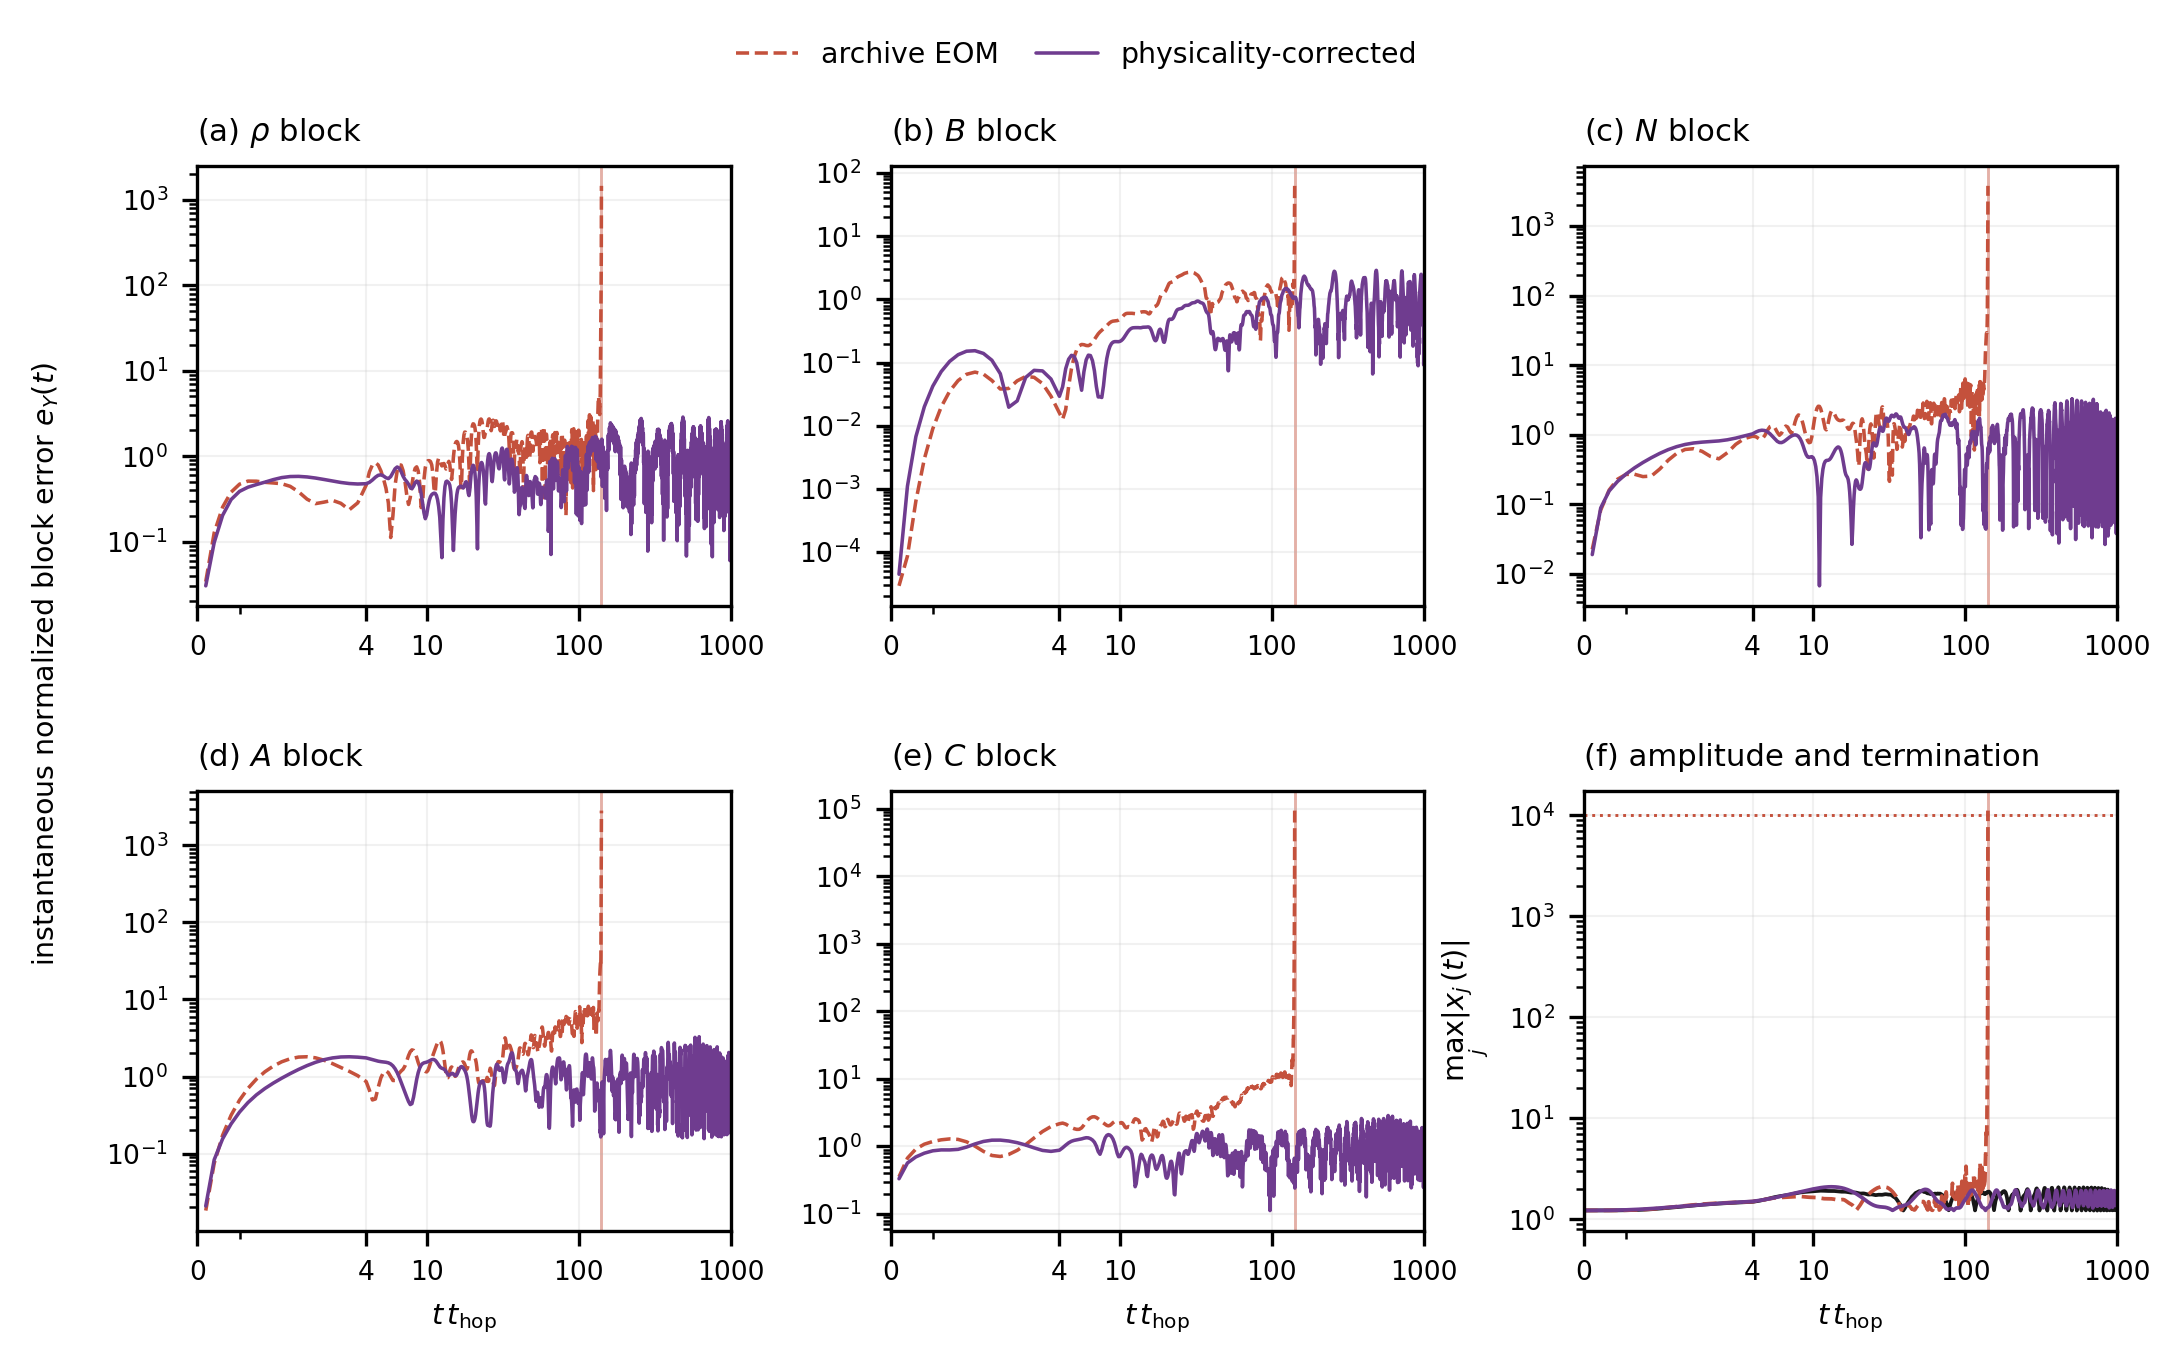
\includegraphics[width=0.98\textwidth]{advisor_project_overview_assets/paper_v/paper_v_block_error_trajectories.pdf}
\caption{Instantaneous dynamic-normalized errors from
Eq.~\eqref{eq:trajectory-error}.  Panels (a)--(e) compare each reconstructed
moment block with the exact cutoff-16 contraction.  Panel (f) shows the
coordinate amplitude, including the $10^4$ declaration threshold.  The raw
curve ends at its numerical-divergence event; no raw values are extrapolated
to $t=1000$.  The expanded early-time scale is linear on $0\leq t\leq4$ and
logarithmic afterward.}
\label{fig:block-error-trajectories}
\end{figure*}

\begin{figure*}[t]
\centering
\includegraphics[width=0.98\textwidth]{advisor_project_overview_assets/paper_v/paper_v_correction_metric_block_errors_t20.pdf}
\caption{Short-time metric ablation.  Panels (a)--(e) show the instantaneous
dynamic-normalized block errors for the raw, Euclidean-corrected, and
lifted-Frobenius-corrected trajectories.  Panel (f) shows
$\lambda_{\min}(\mathcal G)$, including the exact cutoff-16 trajectory in
black; the blue bands mark $0\leq t\leq4$.}
\label{fig:block-error-trajectories-short}
\end{figure*}

At $T=20$, the Euclidean values
$(\varepsilon_\rho,\varepsilon_B,\varepsilon_N,
\varepsilon_A,\varepsilon_C)=(0.4269,0.2193,0.9450,1.3415,0.9530)$ changed
under Eq.~\eqref{eq:frobenius-objective} to
$(0.3972,0.1754,0.8890,1.3975,0.9256)$.  Thus the Frobenius metric reduced
the $\rho$, $B$, $N$, and $C$ errors but increased the $A$ error; the
combined normalized block RMS decreased by only $0.55\%$.  The occupation
RMS error decreased from $0.06091$ to $0.05502$, while the internal-energy
RMS error increased from $0.06284\,t_{\rm hop}$ to
$0.12788\,t_{\rm hop}$.  This does not contradict the zero correction-energy
flux: the changed state path experiences different work from the
time-dependent drive.  Both trajectories remained representable, all
$8{,}000$ constrained evaluations per lane converged, and step halving
changed either trajectory by at most $2.6\times10^{-6}$ in coordinate
$\ell_2$ norm.  The Frobenius metric therefore redistributes the correction
and is not a uniform accuracy improvement.

To localize the closure defect before trajectory separation, exact
wavefunction samples were contracted to $X_{\rm ex}(t)$ and the two local
derivatives were compared at the same state:
\begin{equation}
\dot C_{31}=F_C(t,X_{\rm ex}),\qquad
\dot C_{\rm ex}=\ii\langle[H,\widehat C]\rangle_{\psi_{\rm ex}}.
\label{eq:c-local-comparison}
\end{equation}
For $O_{ij}=c_{j\uparrow}^\dagger c_{i\uparrow}$,
$\delta X_r=\delta b_r+\delta b_r^\dagger$, define
\begin{equation}
\begin{aligned}
Q^{qr}_{ij}&=\langle[O_{ij},n_{r\uparrow}]\delta X_r\delta b_q\rangle,\\
Q^{qr}_{ij,0}&=\langle[O_{ij},n_{r\uparrow}]\rangle
\langle\delta X_r\delta b_q\rangle,\\
K^{qr}_{ij}&=Q^{qr}_{ij}-Q^{qr}_{ij,0},\\
P^q_{ij}&=\delta_{iq}\rho_{qj}-\rho_{ij}\rho_{qq},\\
D^q_{ij}&=\langle O_{ij}n_{q\downarrow}\rangle
-\rho_{ij}\langle n_{q\downarrow}\rangle.
\end{aligned}
\label{eq:kpd-definitions}
\end{equation}
These are, respectively, the omitted connected electron--two-phonon term,
the exact same-spin Pauli covariance, and the omitted opposite-spin
covariance.  Their derivative contributions are
\begin{equation}
\begin{aligned}
\dot C^q_{K,ij}&=-\ii g\sum_rK^{qr}_{ij},\\
\dot C^q_{P,ij}&=-\ii gP^q_{ij}
-\left[(\textstyle\sum_aS_a^q)_{ij}+\ii g\sum_rQ^{qr}_{ij,0}\right],\\
\dot C^q_{D,ij}&=-\ii gD^q_{ij},
\end{aligned}
\label{eq:kpd-velocities}
\end{equation}
where the $P$ term replaces the effective same-spin contribution already in
Eq.~\eqref{eq:eom-c}.  The exact local decomposition is
\begin{equation}
\dot C_{\rm ex}=\dot C_{31}+\dot C_K+\dot C_P
+\dot C_D+R_{\rm cut}.
\label{eq:c-decomposition}
\end{equation}
Let $\mathcal R_C$ extract the 14 real correlation coordinates.  For a set of
supplied terms $S\subseteq\{K,P,D\}$, the initial-residual-subtracted defect
is
{\scriptsize
\begin{equation}
\begin{aligned}
e_S(t)=\mathcal R_C\!\Bigl[&
\dot C_{31}(t)+\sum_{\alpha\in S}\dot C_\alpha(t)-\dot C_{\rm ex}(t)\\
&-\dot C_{31}(0)-\sum_{\alpha\in S}\dot C_\alpha(0)
+\dot C_{\rm ex}(0)\Bigr].
\end{aligned}
\label{eq:c-defect}
\end{equation}}
Over $T=4$, the diagnostic reports
\begin{equation}
\operatorname{RMS}(S)=
\left[\frac1T\int_0^T\norm{e_S(t)}_2^2dt\right]^{1/2},
\label{eq:c-rms}
\end{equation}
with
\begin{table}[H]
\centering
\small
\begin{tabular}{@{}lcc@{}}
\toprule
supplied terms $S$ & RMS & $\max_t\norm{e_S(t)}_2$\\
\midrule
$\varnothing$ & 0.166690 & 0.274310\\
$K$ & 0.089345 & 0.137864\\
$K+P$ & 0.026160 & 0.038268\\
$K+P+D$ & $2.53\times10^{-5}$ & $3.47\times10^{-5}$\\
\bottomrule
\end{tabular}
\caption{Offline reconstruction of the missing $C$ derivative.}
\label{tab:c-attribution}
\end{table}

\begin{figure}[t]
\centering
\includegraphics[width=\columnwidth]{advisor_project_overview_assets/paper_v/paper_v_missing_physics.pdf}
\caption{Exact-state derivative audit.  Higher-order information is supplied
successively to the archive $C$ velocity; the final residual is at the
finite-cutoff scale.}
\label{fig:c-attribution}
\end{figure}

The online right-hand side uses the retained moments and the minimum-norm
correction $w^*$.  The $K,P,D$ quantities in
Eqs.~\eqref{eq:kpd-definitions}--\eqref{eq:c-rms} serve as offline
exact-reference data.  The constrained velocity therefore establishes
representability preservation, while the derivative audit identifies the
additional information required by a more accurate autonomous closure.

\subsection{Autonomous hierarchy extensions}

Dimer symmetry leaves four independent real coordinates in $K$ and three in
$D$; the same-spin term $P$ is algebraically determined by $\rho$.  Appending
these seven coordinates to the archive state gives a 38-coordinate candidate.
Their commutator derivatives generate the remaining cross-spin covariances
and connected one-electron/three-phonon and two-electron/one-phonon moments,
so autonomy requires a larger hierarchy.

For a systematic extension, define
$b_\pm=(b_0\pm b_1)/\sqrt2$, $B_+=(B_0+B_1)/\sqrt2$, and the relative-mode quadratures
$X_-=(b_-+b_-^\dagger)/\sqrt2$ and
$P_-=(b_--b_-^\dagger)/(\ii\sqrt2)$.  The 47- and 82-coordinate candidates
retain spin-exchange-symmetric Hermitian Weyl moments of the form
\begin{equation}
\left\langle\sigma_\mu^\uparrow\sigma_\nu^\downarrow
\,\mathcal W(X_-^aP_-^b)\right\rangle,
\qquad \mu,\nu\in\{I,x,y,z\},
\label{eq:weyl-hierarchy}
\end{equation}
where $\mathcal W$ symmetrizes the phonon quadratures and
$d=\mathbf 1_{\mu\ne I}+\mathbf 1_{\nu\ne I}+a+b$ is the total degree.  If
$m_d$ denotes the real vector of retained degree-$d$ moments, the terminal derivative gate is
the relative time-RMS defect
\begin{equation}
\eta_d=
\frac{[T^{-1}\int_0^T\norm{\dot m_d^{\rm(cl)}-
\dot m_d^{\rm(ex)}}_2^2dt]^{1/2}}
{[T^{-1}\int_0^T\norm{\dot m_d^{\rm(ex)}}_2^2dt]^{1/2}}.
\label{eq:terminal-gate}
\end{equation}
The cutoff-20 audits over $0\leq t\leq4$ give
\begin{table}[H]
\centering
\scriptsize
\begin{tabular}{@{}lp{0.31\columnwidth}p{0.46\columnwidth}@{}}
\toprule
state & retained extension & terminal result\\
\midrule
38 & archive 31 plus four $K$ and three $D$ coordinates
& their derivatives generate additional moments\\
47 & $B_+$ and all symmetry-adapted moments through degree three
& zero connected fourth cumulant gives $\eta_3=0.7302$\\
82 & 47 coordinates plus all 35 degree-four moments
& zero connected fifth cumulant gives $\eta_4=2.1276$\\
\bottomrule
\end{tabular}
\caption{Autonomous hierarchy-extension gates.}
\label{tab:hierarchy-gates}
\end{table}
Each extension makes the previously terminal equations accurate: the
47-coordinate equations reduce the projected $C$-velocity RMS defect to
$1.01\times10^{-6}$, and the 82-coordinate equations reduce the former
degree-three relative defect to $5.45\times10^{-6}$.  The dominant error
moves to the newly highest-order block.  A convergent autonomous model thus
requires a physically adapted approximation for its terminal moments, rather
than direct order-by-order zero-cumulant truncation.

\clearpage
\appendix

\section{Gram positivity and Schur reduction}
\label{app:gram-schur}

Partition $z=(u,v)$ with $u\in\C^4$ and $v\in\C^3$.  The block matrix in
Eq.~\eqref{eq:joint-gram} gives
\begin{equation}
z^\dagger\mathcal Gz
=u^\dagger\MB u+u^\dagger Zv+v^\dagger Z^\dagger u+v^\dagger Ev.
\label{eq:app-block-form}
\end{equation}
The operator row in Eq.~\eqref{eq:operator-row} converts this quadratic form
into
\begin{equation}
z^\dagger\mathcal Gz
=\left\langle\left(\sum_a z_aY_a\right)^\dagger
\left(\sum_b z_bY_b\right)\right\rangle,
\label{eq:app-gram-form}
\end{equation}
which is nonnegative for every $z$.  Choosing $v=0$ gives
$u^\dagger\MB u\geq0$ and proves principal-submatrix inheritance directly.
For $\MB\succ0$, completing the square in Eq.~\eqref{eq:app-block-form}
gives~\cite{zhang2005}
\begin{equation}
\begin{aligned}
z^\dagger\mathcal Gz={}&
(u+\MB^{-1}Zv)^\dagger\MB(u+\MB^{-1}Zv)\\
&+v^\dagger(E-Z^\dagger\MB^{-1}Z)v.
\end{aligned}
\label{eq:app-square}
\end{equation}
The first term is positive for every $u$; minimizing it at
$u=-\MB^{-1}Zv$ leaves the Schur complement in
Eq.~\eqref{eq:schur}.  This establishes the equivalence between joint Gram
positivity and the marginal-plus-cross-correlation condition.

\section{Origin of the correction constraints}
\label{app:constraint-origin}

For a constrained Hermitian matrix $M(x)$, an online coordinate correction
$w$ changes its velocity from $\dot M_0$ to
$\dot M_{\rm c}=\dot M_0+\Delta\dot M(w)$.  Substitution into
Eq.~\eqref{eq:matrix-barrier} gives
\begin{equation}
\dot M_0+\Delta\dot M(w)+\beta(M-h_\star I)\succeq0.
\label{eq:app-generic-barrier}
\end{equation}
Applying Eq.~\eqref{eq:app-generic-barrier} to $M=\rho$, $M=I_2-\rho$,
and $M=\mathcal G$ gives the first three constraint lines of
Eq.~\eqref{eq:correction-sdp}; the upper electronic boundary uses
$d(I_2-\rho)/dt=-\dot\rho$.

For the shared correlation trace $s=\Tr C^q$, exponential restoration to the
fixed-number manifold is $\dot s_{\rm c}+\beta s=0$.  Since the lifted
coordinates satisfy
$\Delta\dot s(w)=w_{17}+\ii w_{18}$, this is the fourth constraint line and
the last two rows of Eq.~\eqref{eq:equality-system}.  Finally, the chain rule
gives the instantaneous energy change induced by the correction,
\begin{equation}
\left.\frac{dE_{\rm int}}{dt}\right|_{w}
=\nabla_xE_{\rm int}(x)^\mathsf Tw.
\label{eq:app-energy-chain-rule}
\end{equation}
Setting Eq.~\eqref{eq:app-energy-chain-rule} to zero gives the final
constraint and the first row of Eq.~\eqref{eq:equality-system}.  The solver
therefore changes the Runge--Kutta stage velocity while preserving the
current reconstructed state at that right-hand-side evaluation.

\begin{thebibliography}{9}
\raggedright

\bibitem{riva2026}
G.~Riva, J.~Simoni, and Y.~Ping,
``Open-quantum-system theory of non-Markovian electron--phonon dynamics,''
arXiv:2606.22233 (2026).

\bibitem{hornJohnson2012}
R.~A. Horn and C.~R. Johnson,
\emph{Matrix Analysis}, 2nd ed. (Cambridge University Press, Cambridge,
2012), doi:10.1017/CBO9781139020411.

\bibitem{zhang2005}
F.~Zhang, ed., \emph{The Schur Complement and Its Applications}
(Springer, New York, 2005), doi:10.1007/b105056.

\bibitem{kato1966}
T.~Kato, \emph{Perturbation Theory for Linear Operators}
(Springer, Berlin, 1966), doi:10.1007/978-3-662-12678-3.

\bibitem{ong2025}
P.~Ong, Y.~Xu, R.~M.~Bena, F.~Jabbari, and A.~D.~Ames,
``Matrix control barrier functions,'' arXiv:2508.11795v2 (2025),
doi:10.48550/arXiv.2508.11795.

\bibitem{vandenbergheBoyd1996}
L.~Vandenberghe and S.~Boyd, ``Semidefinite programming,''
SIAM Rev. \textbf{38}, 49--95 (1996), doi:10.1137/1038003.

\bibitem{boydVandenberghe2004}
S.~Boyd and L.~Vandenberghe, \emph{Convex Optimization}
(Cambridge University Press, Cambridge, 2004).

\bibitem{hairer1993}
E.~Hairer, S.~P. N\o rsett, and G.~Wanner,
\emph{Solving Ordinary Differential Equations I: Nonstiff Problems},
2nd ed. (Springer, Berlin, 1993), doi:10.1007/978-3-540-78862-1.

\end{thebibliography}

\end{document}
